%
%
%
\begin{figure}[ht]
	\begin{center}
		\begin {tabular}{c}
			\begin{minipage}{8cm}
				\begin{center}
					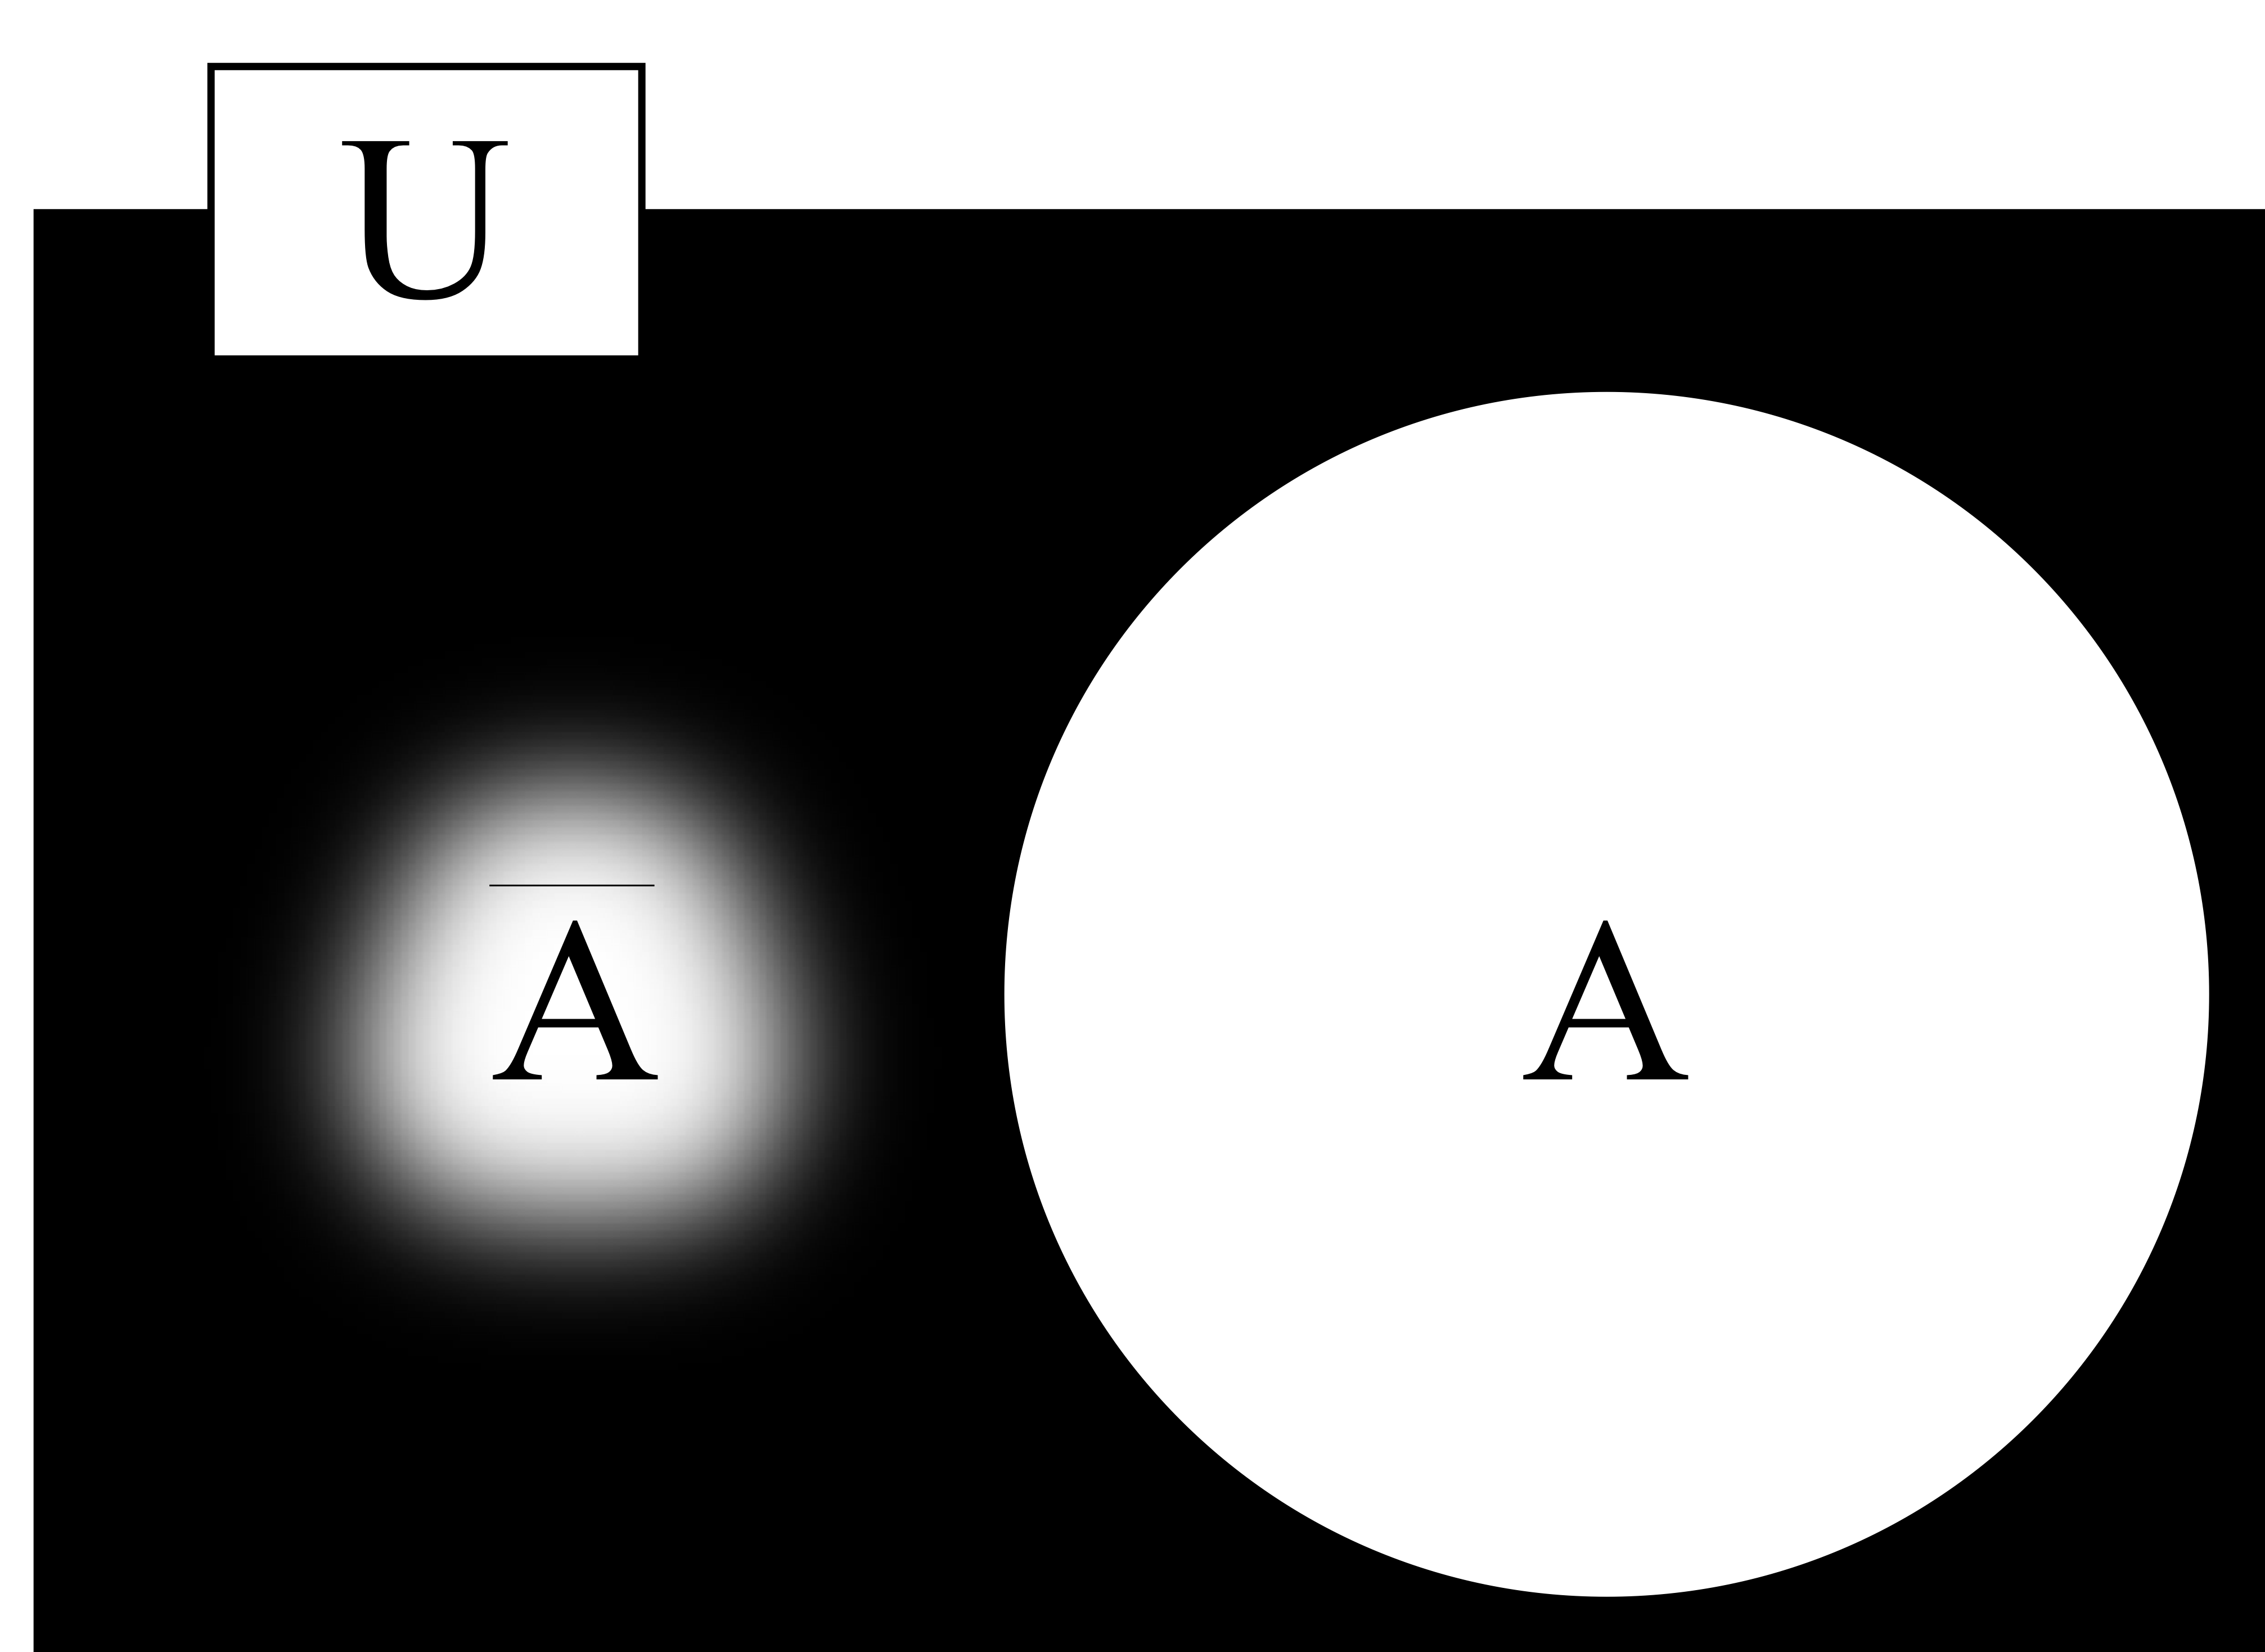
\includegraphics[width=8cm]{v1not.eps} \\%%% ファイル名
				\end {center}
			\end{minipage}
		\end{tabular}
		\caption{補集合のベン図}%%% 表題
		\label{fig:v1not}%%% ラベル
	\end{center}
\end{figure}
%
%
%
\begin{figure}[ht]
	\begin{center}
		\begin {tabular}{c}
			\begin{minipage}{8cm}
				\begin{center}
					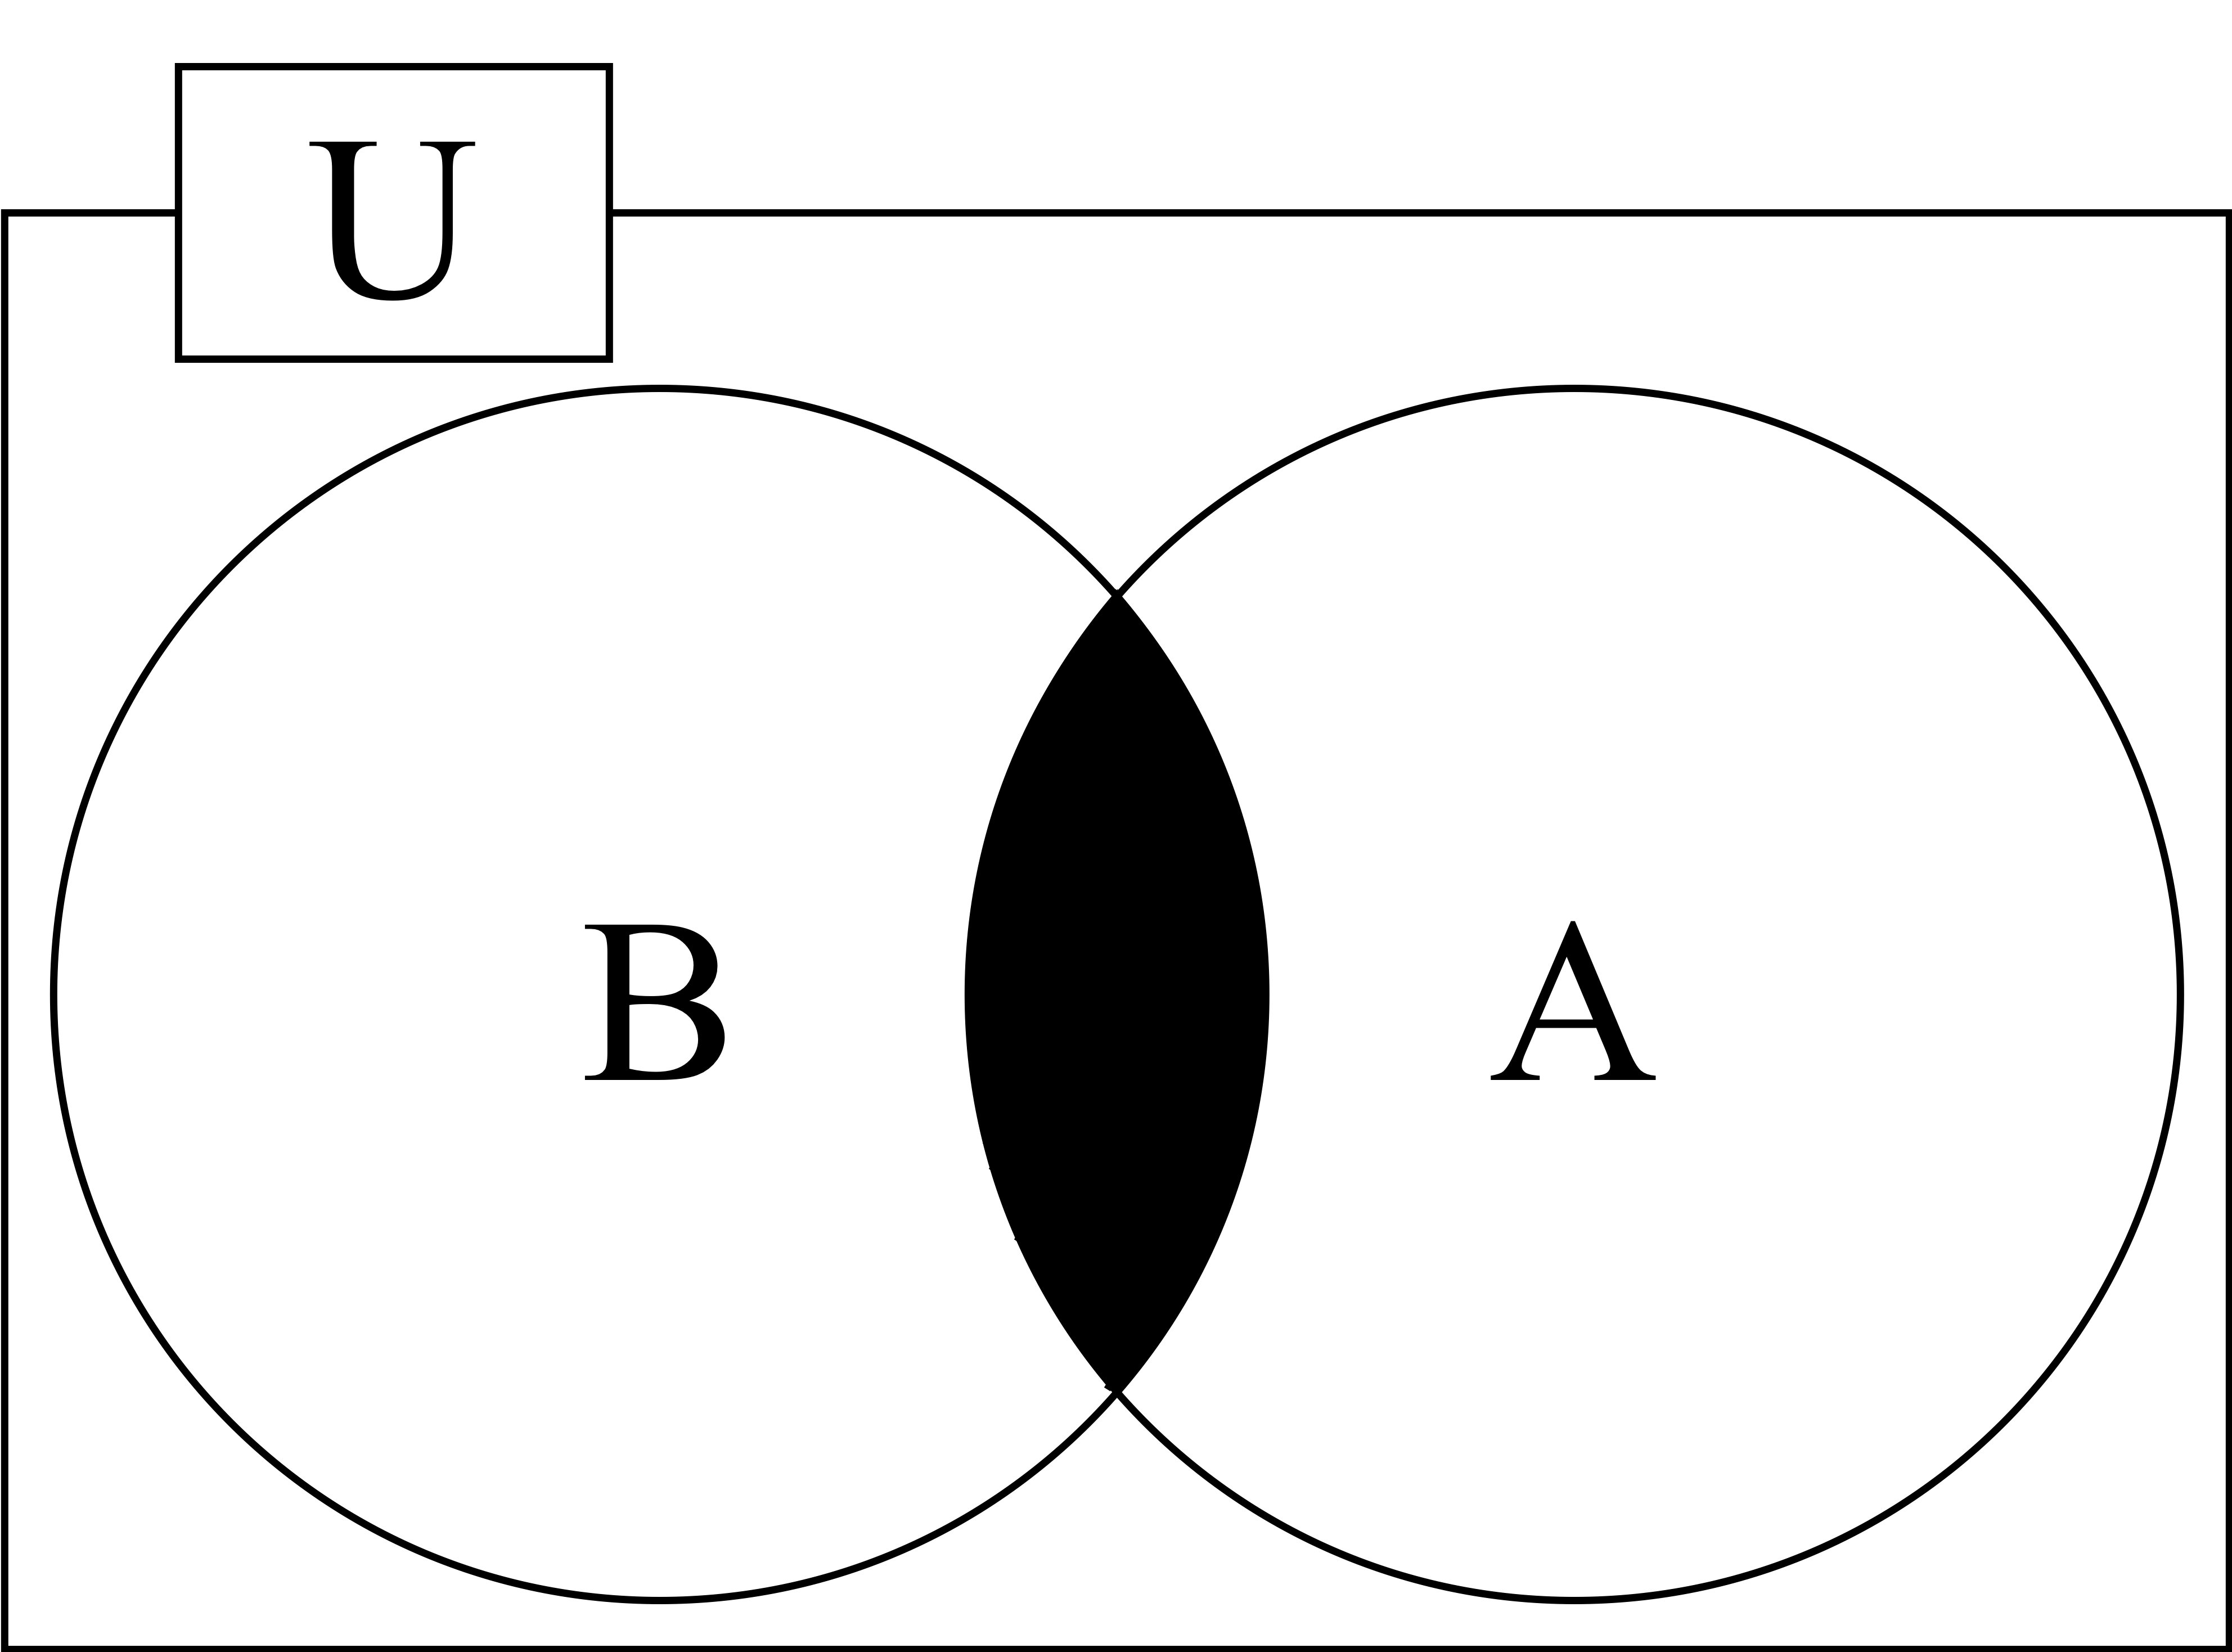
\includegraphics[width=8cm]{v2and.eps} \\%%% ファイル名
				\end {center}
			\end{minipage}
		\end{tabular}
		\caption{積集合のベン図}%%% 表題
		\label{fig:v2and}%%% ラベル
	\end{center}
\end{figure}
%
%
%
\begin{figure}[ht]
	\begin{center}
		\begin {tabular}{c}
			\begin{minipage}{8cm}
				\begin{center}
					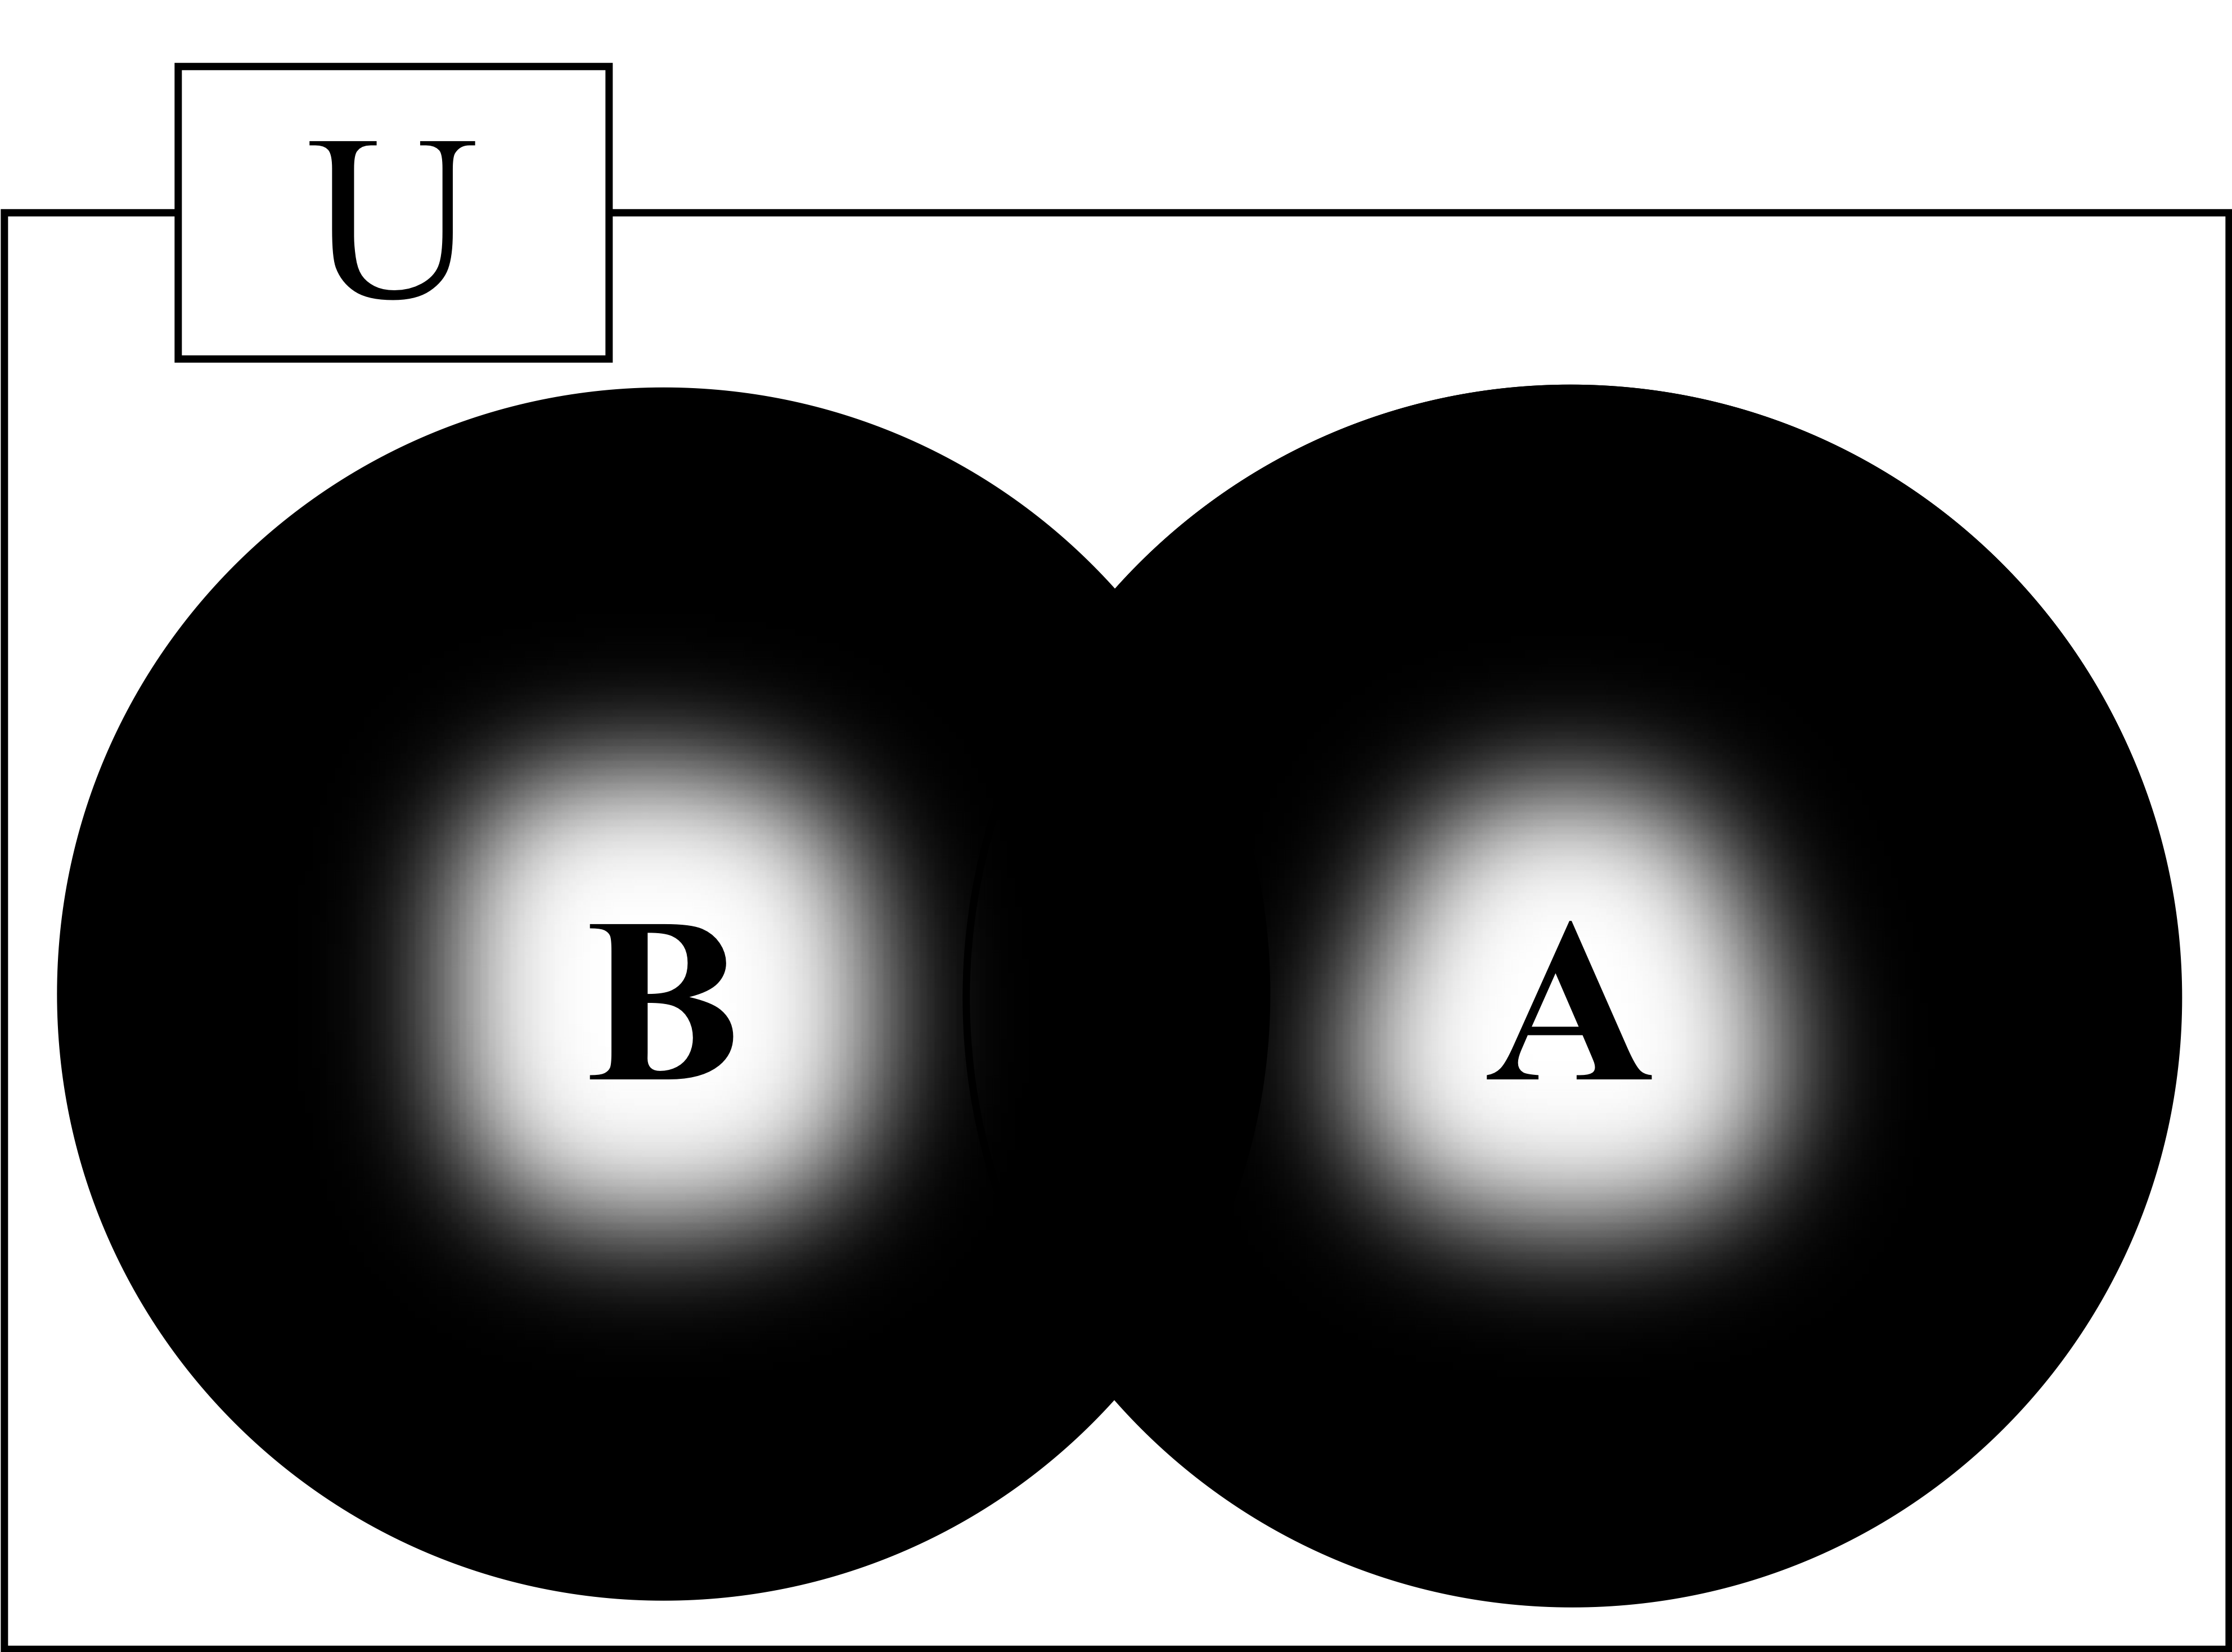
\includegraphics[width=8cm]{v3or.eps} \\%%% ファイル名
				\end {center}
			\end{minipage}
		\end{tabular}
		\caption{和集合のベン図}%%% 表題
		\label{fig:v3or}%%% ラベル
	\end{center}
\end{figure}
%
%
%
\begin{figure}[ht]
	\begin{center}
		\begin {tabular}{c}
			\begin{minipage}{8cm}
				\begin{center}
					\includegraphics[width=8cm]{v4nand.eps} \\%%% ファイル名
				\end {center}
			\end{minipage}
		\end{tabular}
		\caption{積集合の補集合のベン図}%%% 表題
		\label{fig:v4nand}%%% ラベル
	\end{center}
\end{figure}
%
%
%
\begin{figure}[ht]
	\begin{center}
		\begin {tabular}{c}
			\begin{minipage}{8cm}
				\begin{center}
					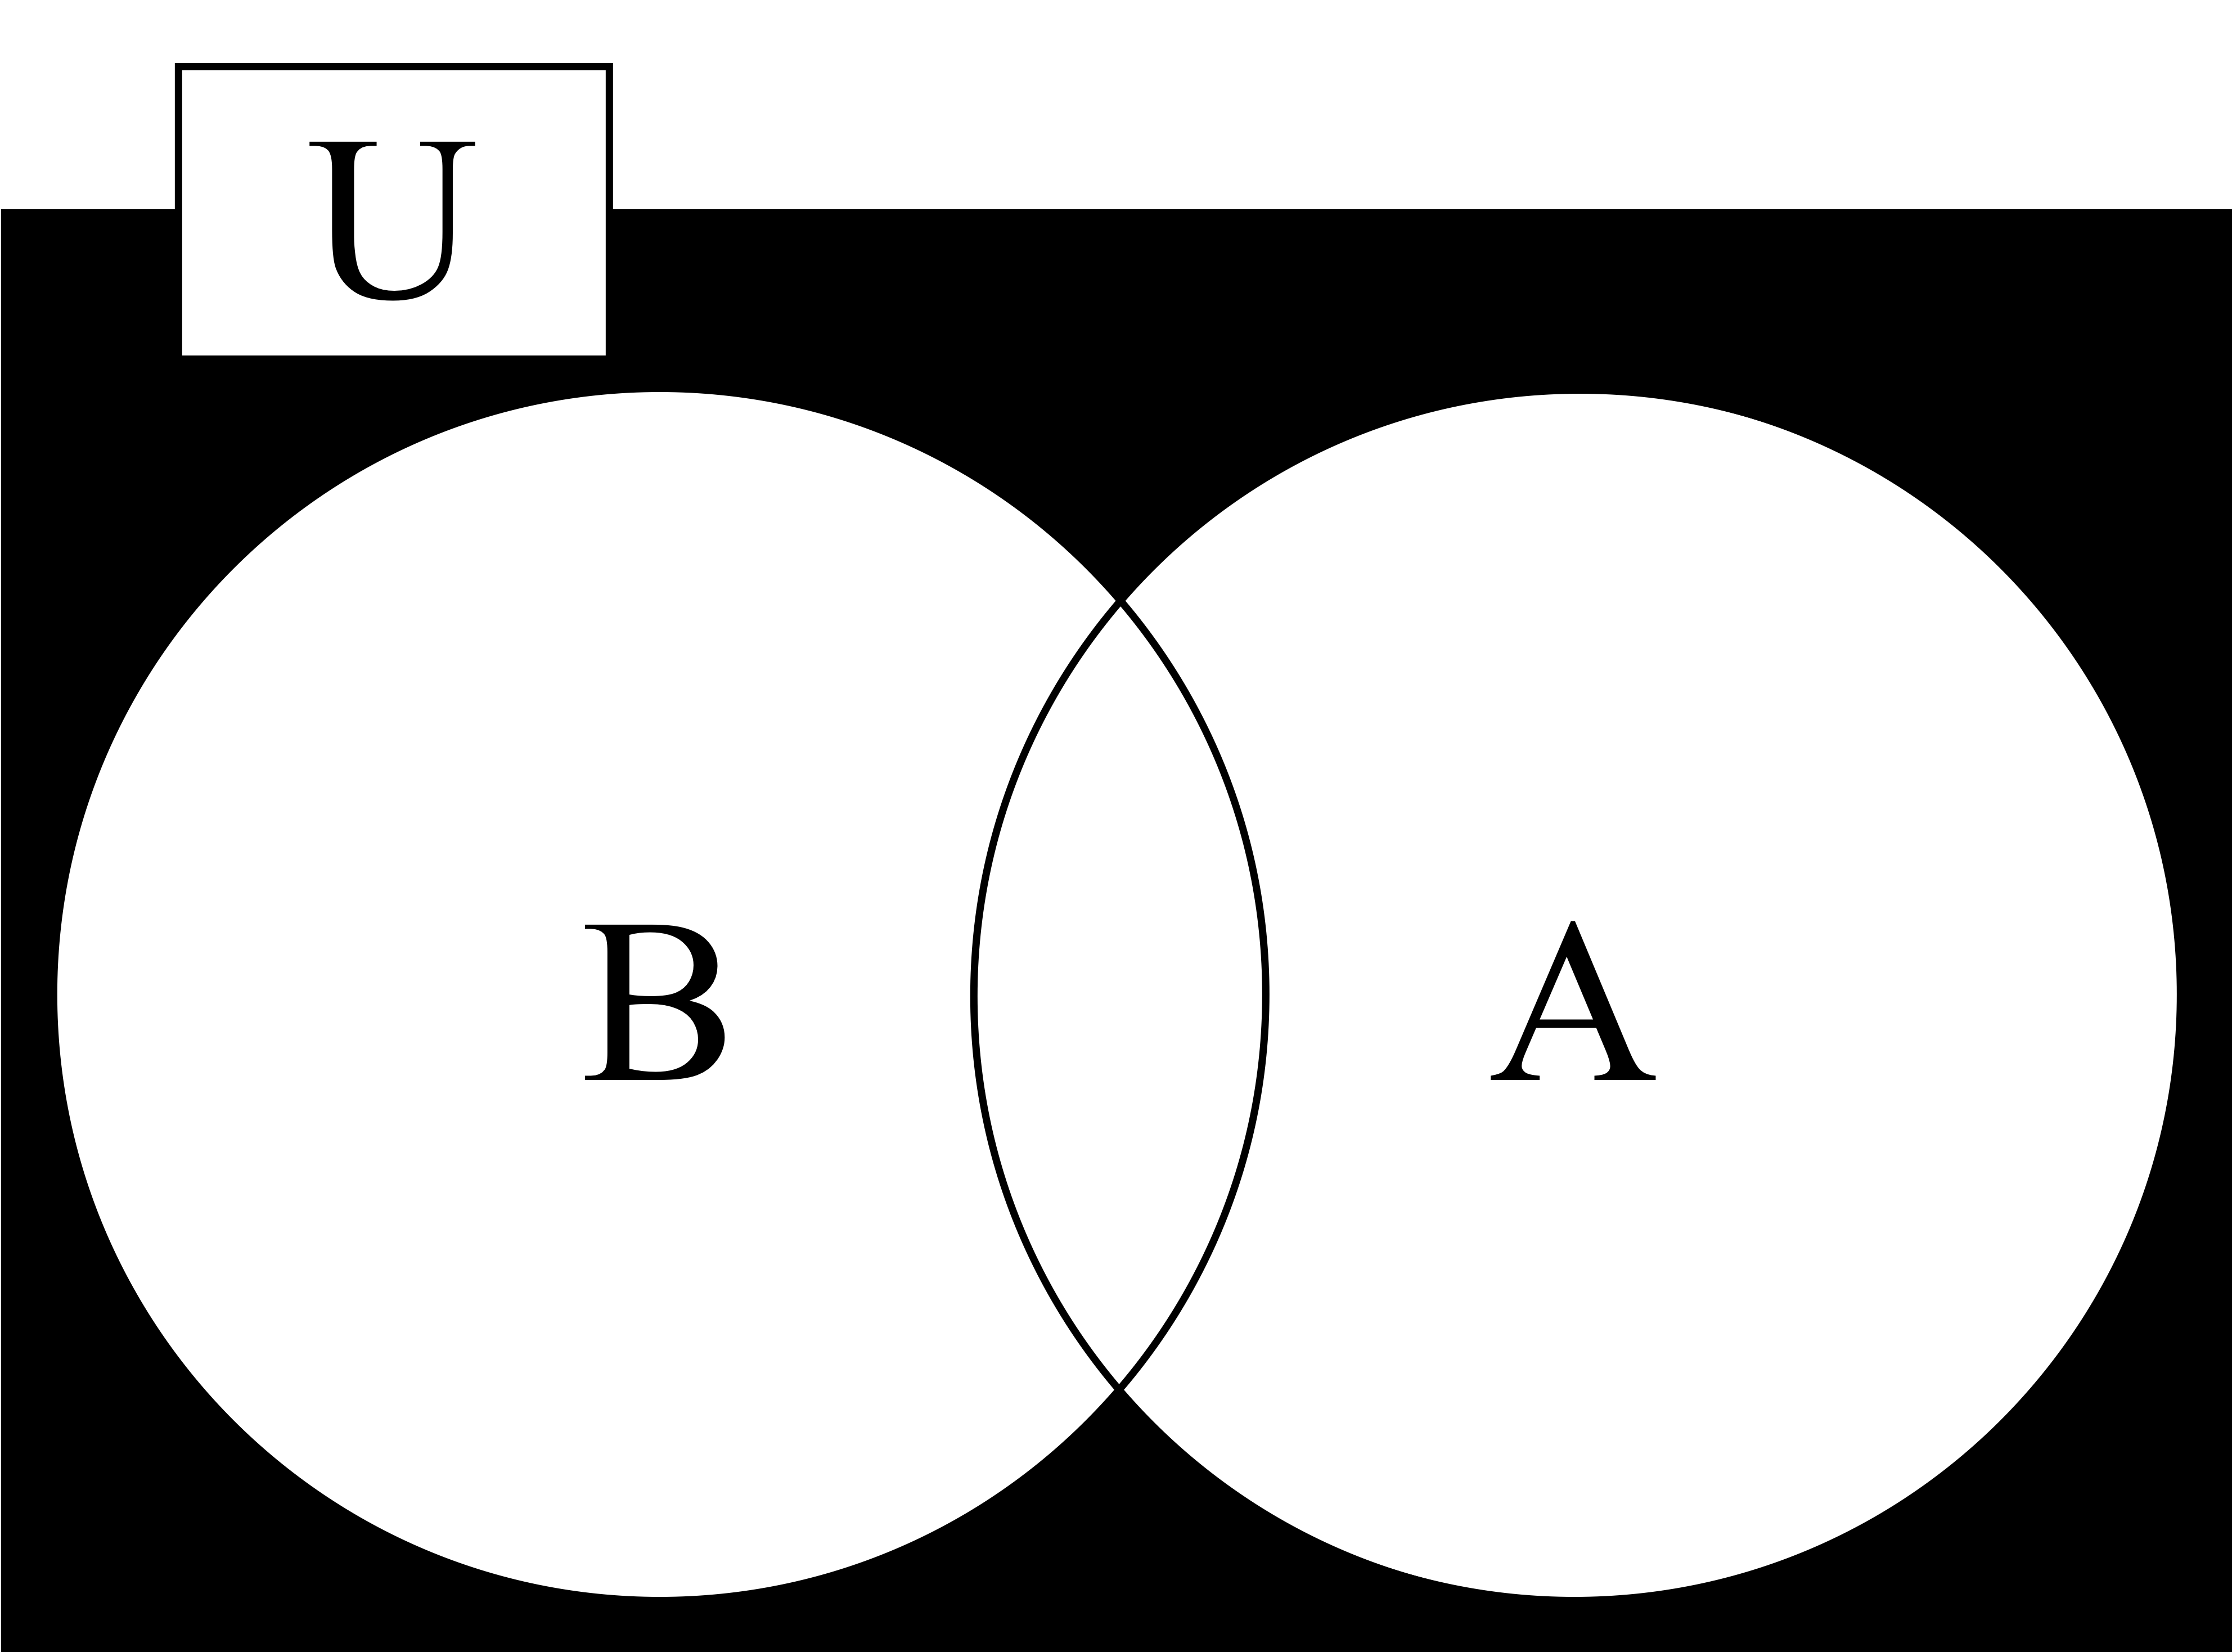
\includegraphics[width=8cm]{v5nor.eps} \\%%% ファイル名
				\end {center}
			\end{minipage}
		\end{tabular}
		\caption{和集合の補集合ベン図}%%% 表題
		\label{fig:v5nor}%%% ラベル
	\end{center}
\end{figure}
%
%
%
\begin{figure}[ht]
	\begin{center}
		\begin {tabular}{c}
			\begin{minipage}{8cm}
				\begin{center}
					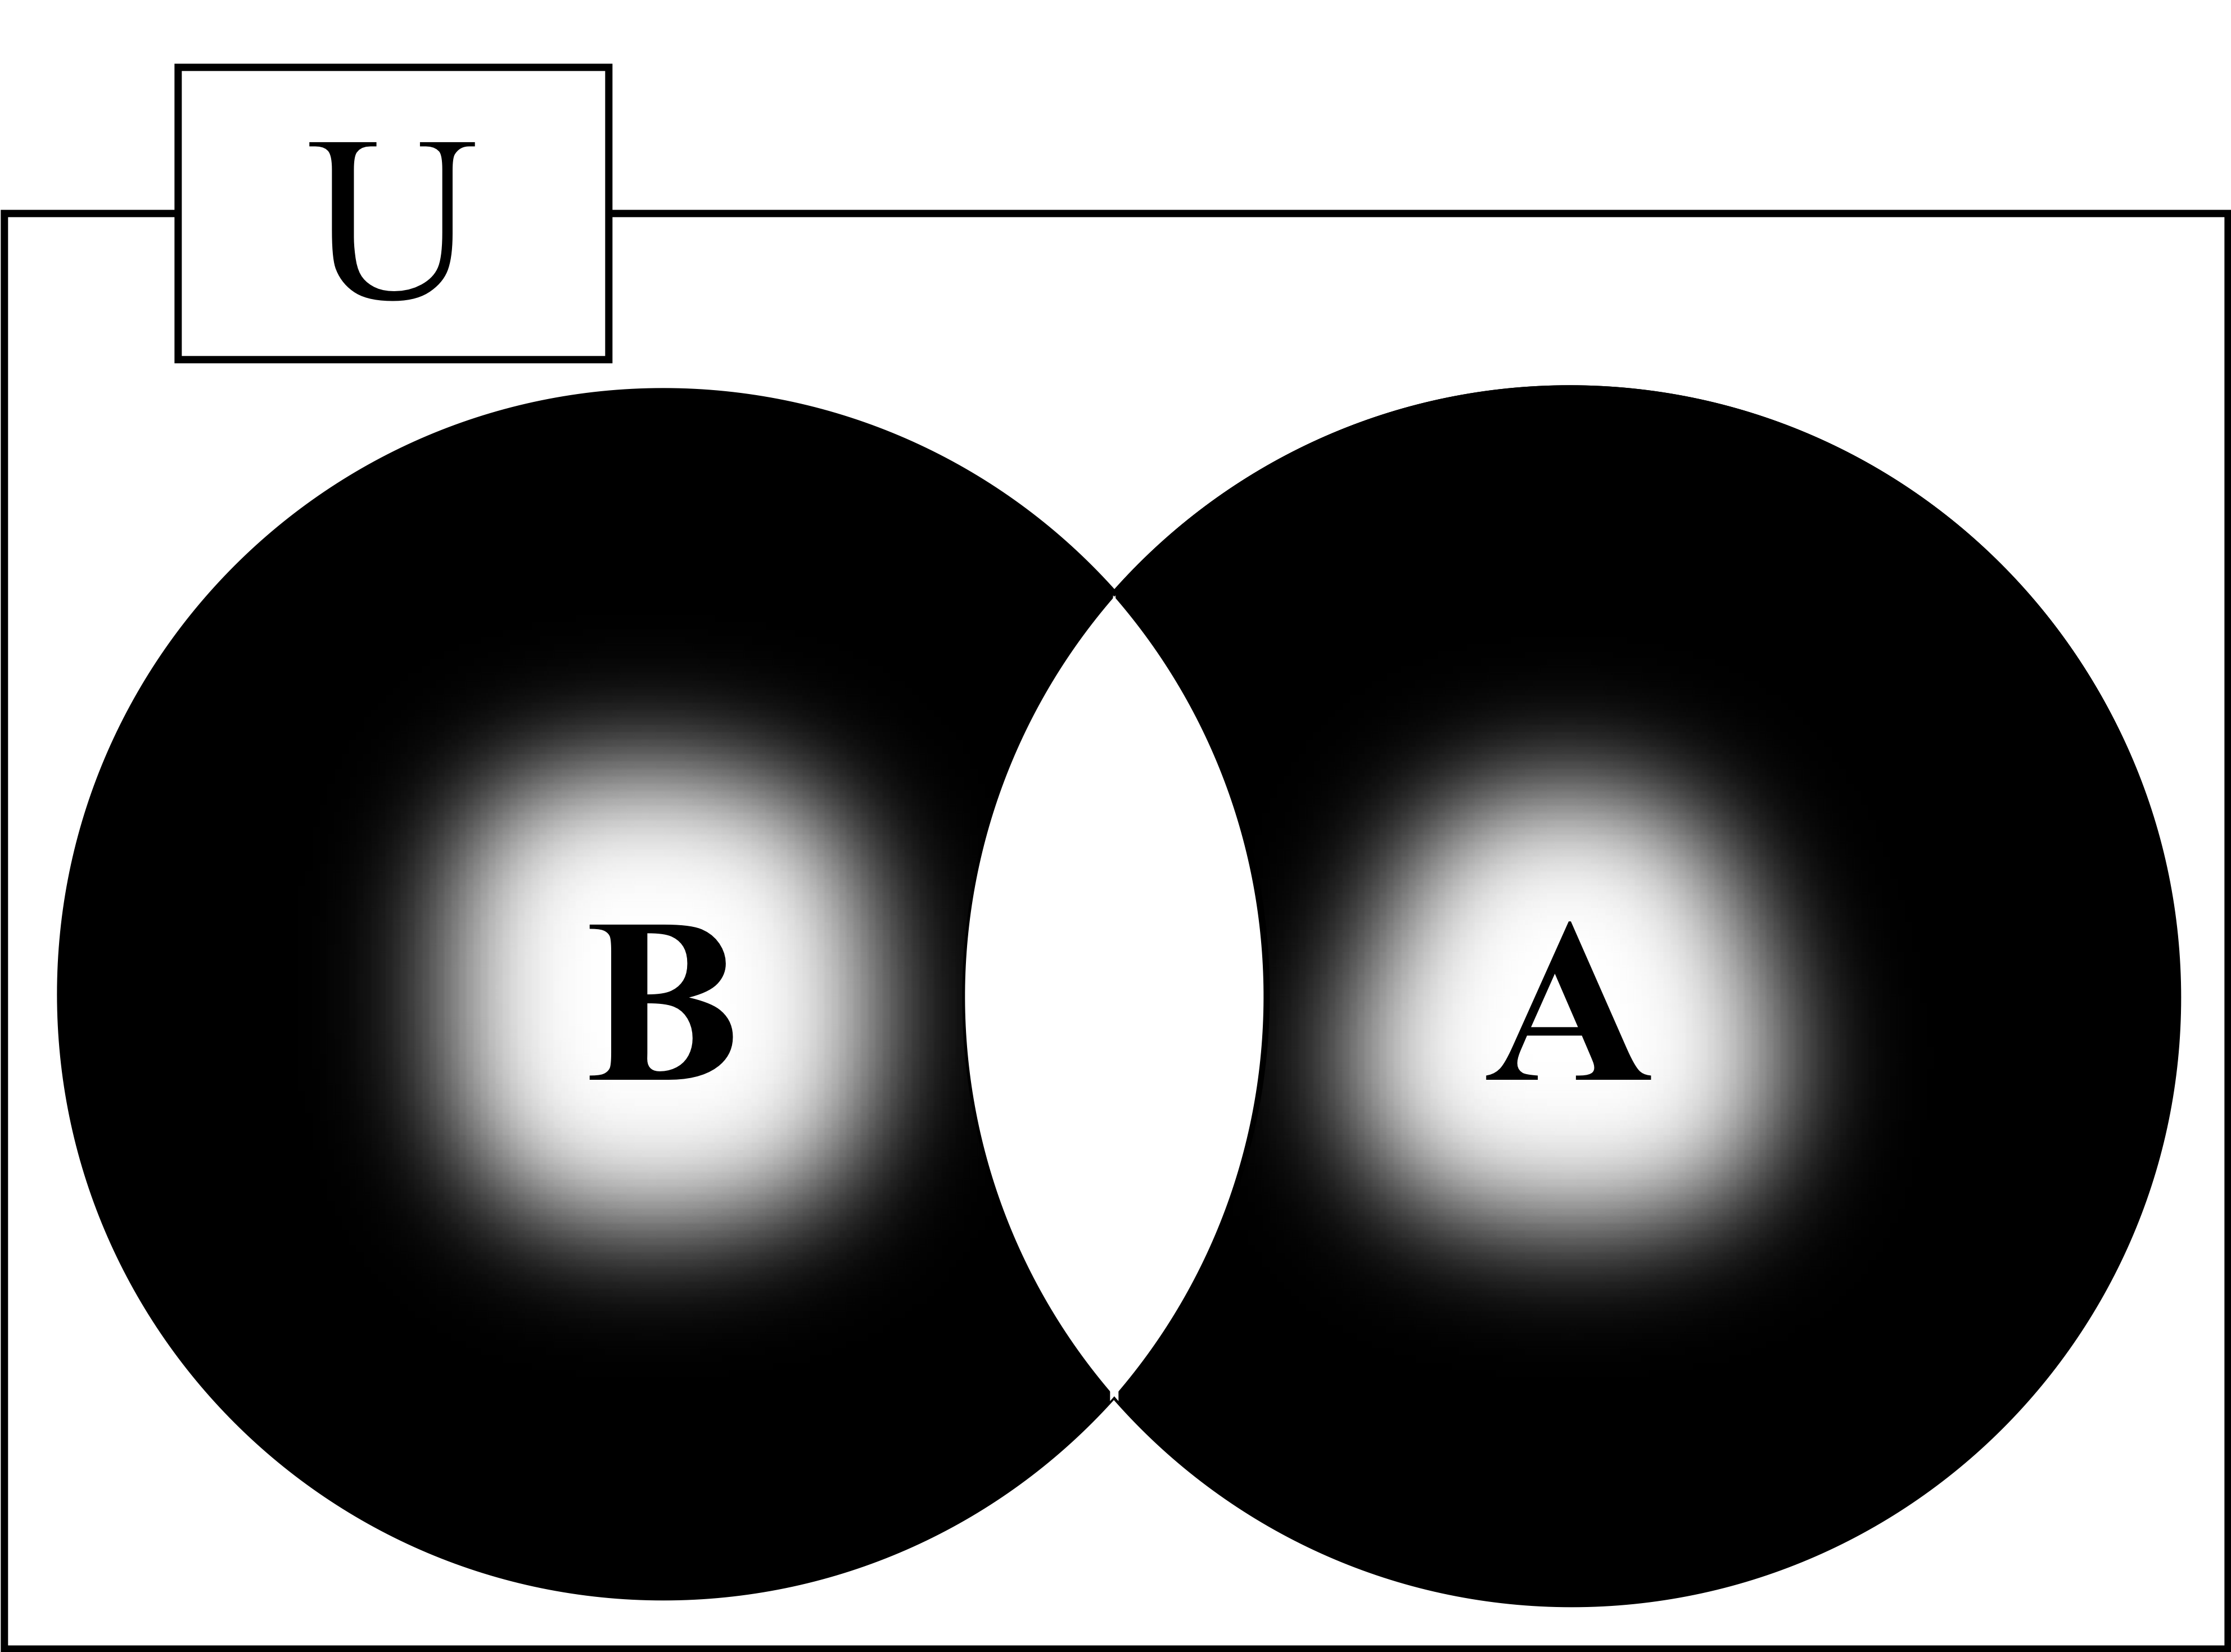
\includegraphics[width=8cm]{v6exor.eps} \\%%% ファイル名
				\end {center}
			\end{minipage}
		\end{tabular}
		\caption{排他的論理和のベン図}%%% 表題
		\label{fig:v6exor}%%% ラベル
	\end{center}
\end{figure}
%
%
%
\begin{figure}[ht]
	\begin{center}
		\begin {tabular}{c}
			\begin{minipage}{8cm}
				\begin{center}
					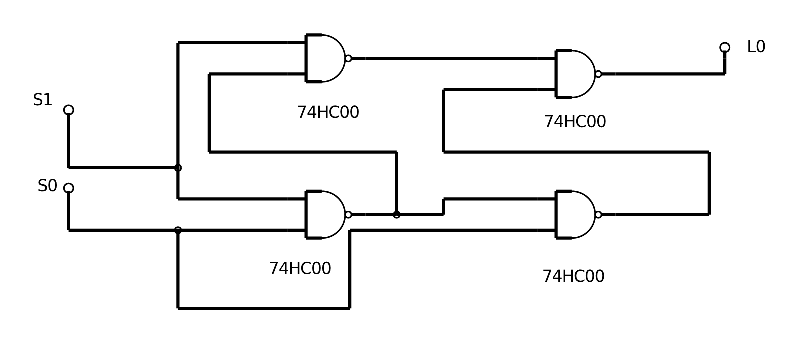
\includegraphics[width=8cm]{exor} \\%%% ファイル名
				\end {center}
			\end{minipage}
		\end{tabular}
		\caption{$2$入力ExOR回路の回路図}%%% 表題
		\label{fig:ExOR}%%% ラベル
	\end{center}
\end{figure}
%
%
%
\begin{figure}[ht]
	\begin{center}
		\begin {tabular}{c}
			\begin{minipage}{8cm}
				\begin{center}
					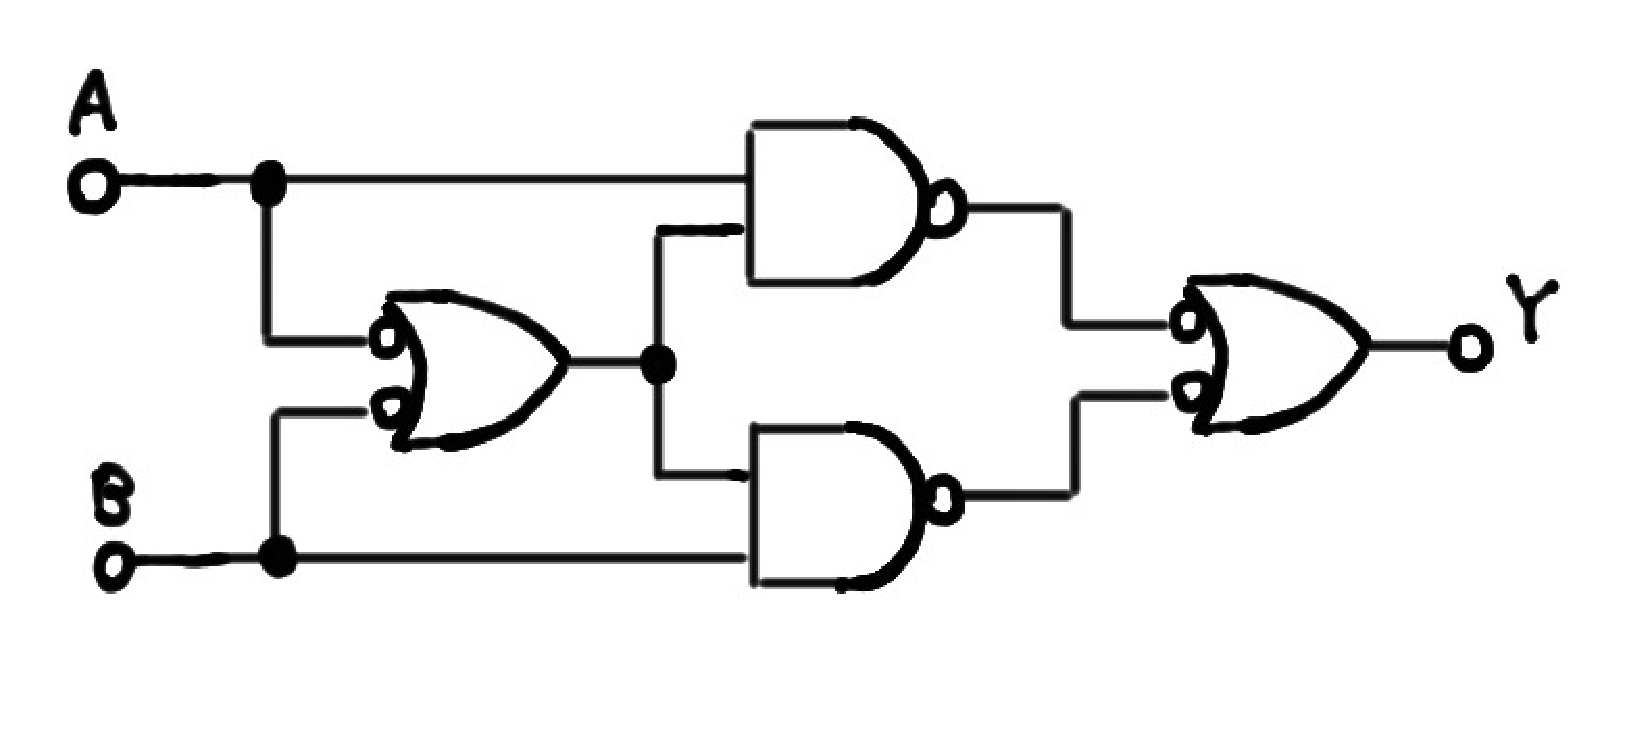
\includegraphics[width=8cm]{exor22} \\%%% ファイル名
				\end {center}
			\end{minipage}
		\end{tabular}
		\caption{課題1におけるExOR回路の回路図}%%% 表題
		\label{fig:ExOR_kadai1}%%% ラベル
	\end{center}
\end{figure}
%
%
%
\begin{figure}[ht]
	\begin{center}
		\begin {tabular}{c}
			\begin{minipage}{8cm}
				\begin{center}
					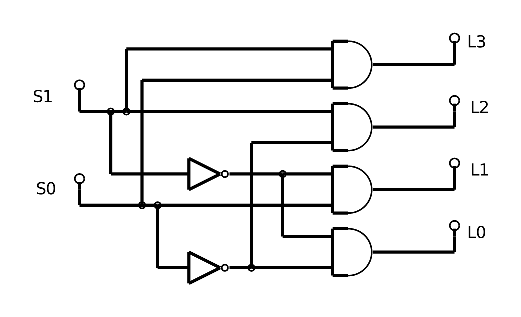
\includegraphics[width=8cm]{24decoder} \\%%% ファイル名
				\end {center}
			\end{minipage}
		\end{tabular}
		\caption{$2$入力$4$出力デコーダの回路図}%%% 表題
		\label{fig:24decoder}%%% ラベル
	\end{center}
\end{figure}
%
%
%
\begin{figure}[ht]
	\begin{center}
		\begin {tabular}{c}
			\begin{minipage}{8cm}
				\begin{center}
					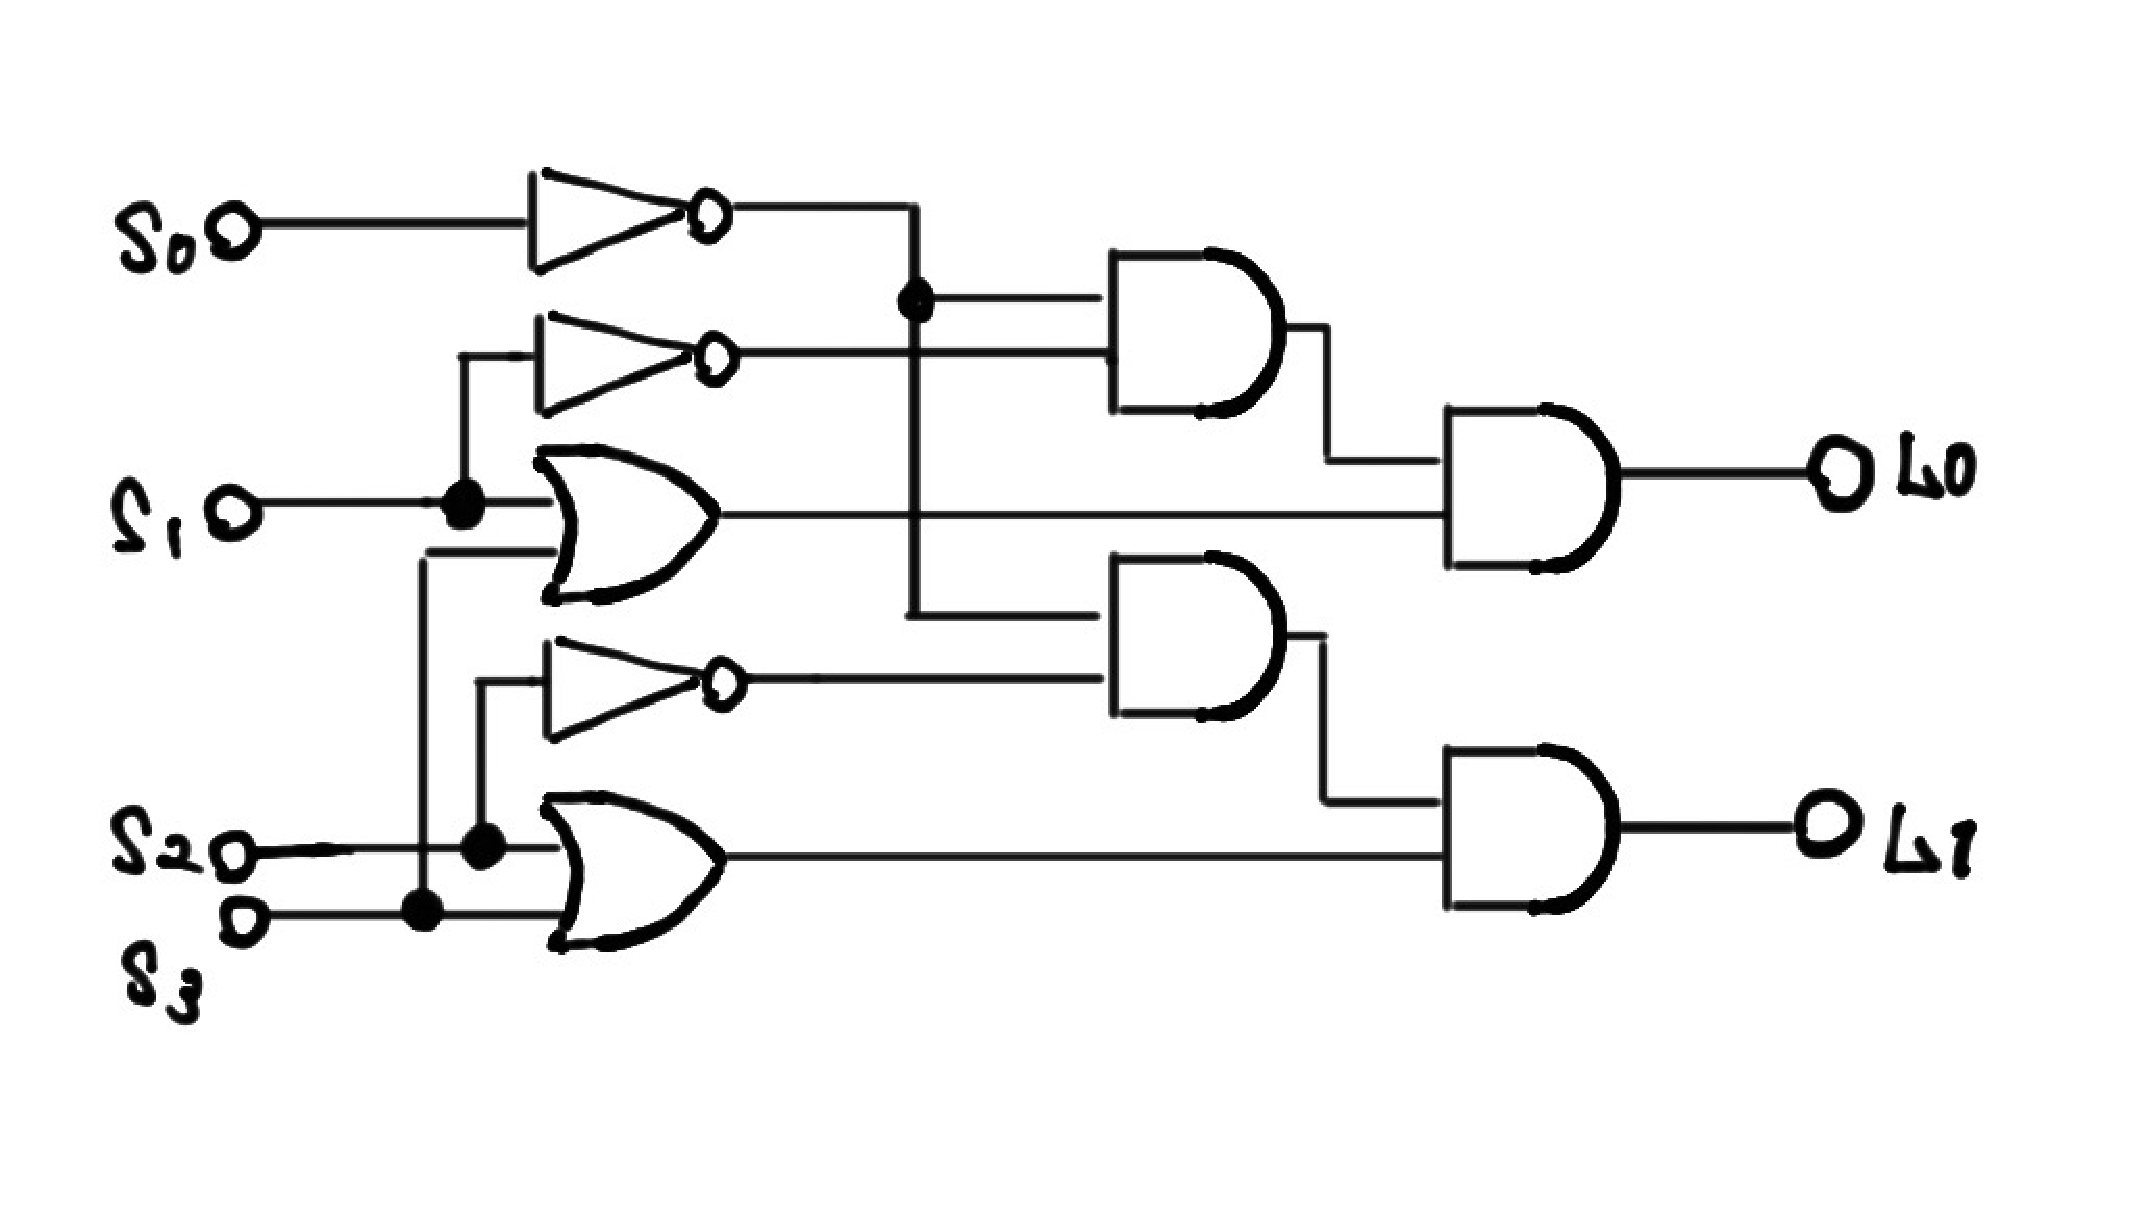
\includegraphics[width=8cm]{halfadder3} \\%%% ファイル名
				\end {center}
			\end{minipage}
		\end{tabular}
		\caption{$4$入力$2$出力エンコーダの回路図(複数選択可能)}%%% 表題
		\label{fig:42encodern}%%% ラベル
	\end{center}
\end{figure}

\begin{figure}[ht]
	\begin{center}
		\begin {tabular}{c}
			\begin{minipage}{8cm}
				\begin{center}
					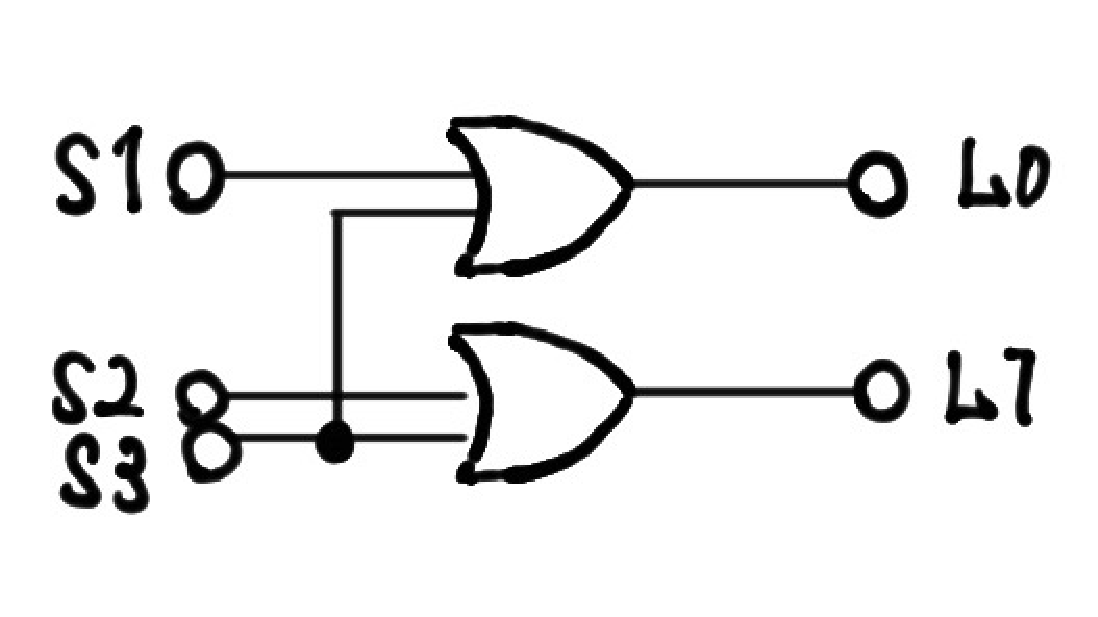
\includegraphics[width=8cm]{halfadder2} \\%%% ファイル名
				\end {center}
			\end{minipage}
		\end{tabular}
		\caption{$4$入力$2$出力エンコーダの回路図(選択が1つしかできない場合)}%%% 表題
		\label{fig:42encoder1}%%% ラベル
	\end{center}
\end{figure}
%
%
%
\begin{figure}[ht]
	\begin{center}
		\begin {tabular}{c}
			\begin{minipage}{8cm}
				\begin{center}
					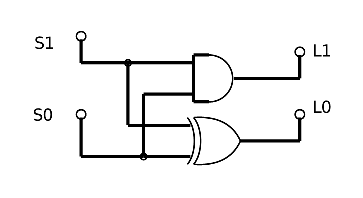
\includegraphics[width=8cm]{halfadder} \\%%% ファイル名
				\end {center}
			\end{minipage}
		\end{tabular}
		\caption{半加算器回路の回路図}%%% 表題
		\label{fig:halfAdder}%%% ラベル
	\end{center}
\end{figure}
%
%
%
\begin{figure}[ht]
	\begin{center}
		\begin {tabular}{c}
			\begin{minipage}{8cm}
				\begin{center}
					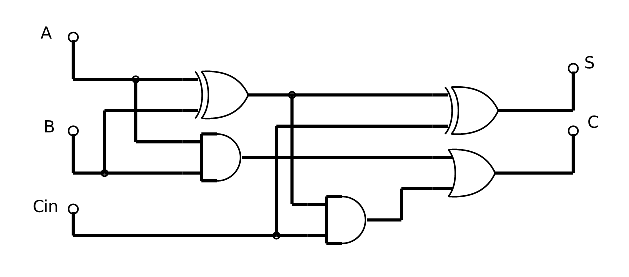
\includegraphics[width=8cm]{fulladder} \\%%% ファイル名
				\end {center}
			\end{minipage}
		\end{tabular}
		\caption{全加算器回路の回路図}%%% 表題
		\label{fig:fullAdder}%%% ラベル
	\end{center}
\end{figure}
%
%
%
\begin{figure}[ht]
	\begin{center}
		\begin {tabular}{c}
			\begin{minipage}{8cm}
				\begin{center}
					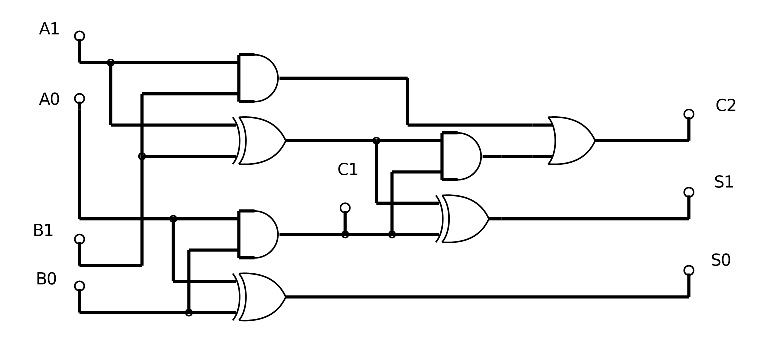
\includegraphics[width=8cm]{22adder} \\%%% ファイル名
				\end {center}
			\end{minipage}
		\end{tabular}
		\caption{2桁の2進数の加算器回路の回路図}%%% 表題
		\label{fig:22Adder}%%% ラベル
	\end{center}
\end{figure}
%
%
%
\begin{figure}[ht]
	\begin{center}
		\begin {tabular}{c}
			\begin{minipage}{8cm}
				\begin{center}
					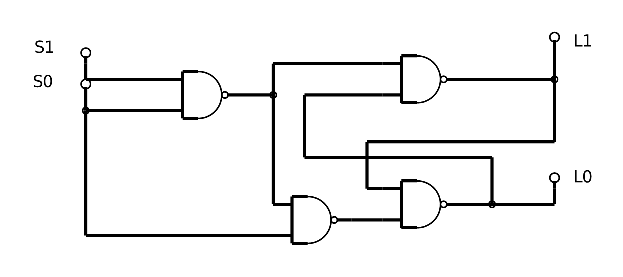
\includegraphics[width=8cm]{Dlatch} \\%%% ファイル名
				\end {center}
			\end{minipage}
		\end{tabular}
		\caption{Dラッチ回路の回路図}%%% 表題
		\label{fig:DLatch}%%% ラベル
	\end{center}
\end{figure}
%
%
%
\begin{figure}[ht]
	\begin{center}
		\begin {tabular}{c}
			\begin{minipage}{8cm}
				\begin{center}
					\includegraphics[width=8cm]{DlatchTC} \\%%% ファイル名
				\end {center}
			\end{minipage}
		\end{tabular}
		\caption{Dラッチ回路のタイムチャート}%%% 表題
		\label{fig:DLatchTC}%%% ラベル
	\end{center}
\end{figure}
%
%
%
\begin{figure}[ht]
	\begin{center}
		\begin {tabular}{c}
			\begin{minipage}{8cm}
				\begin{center}
					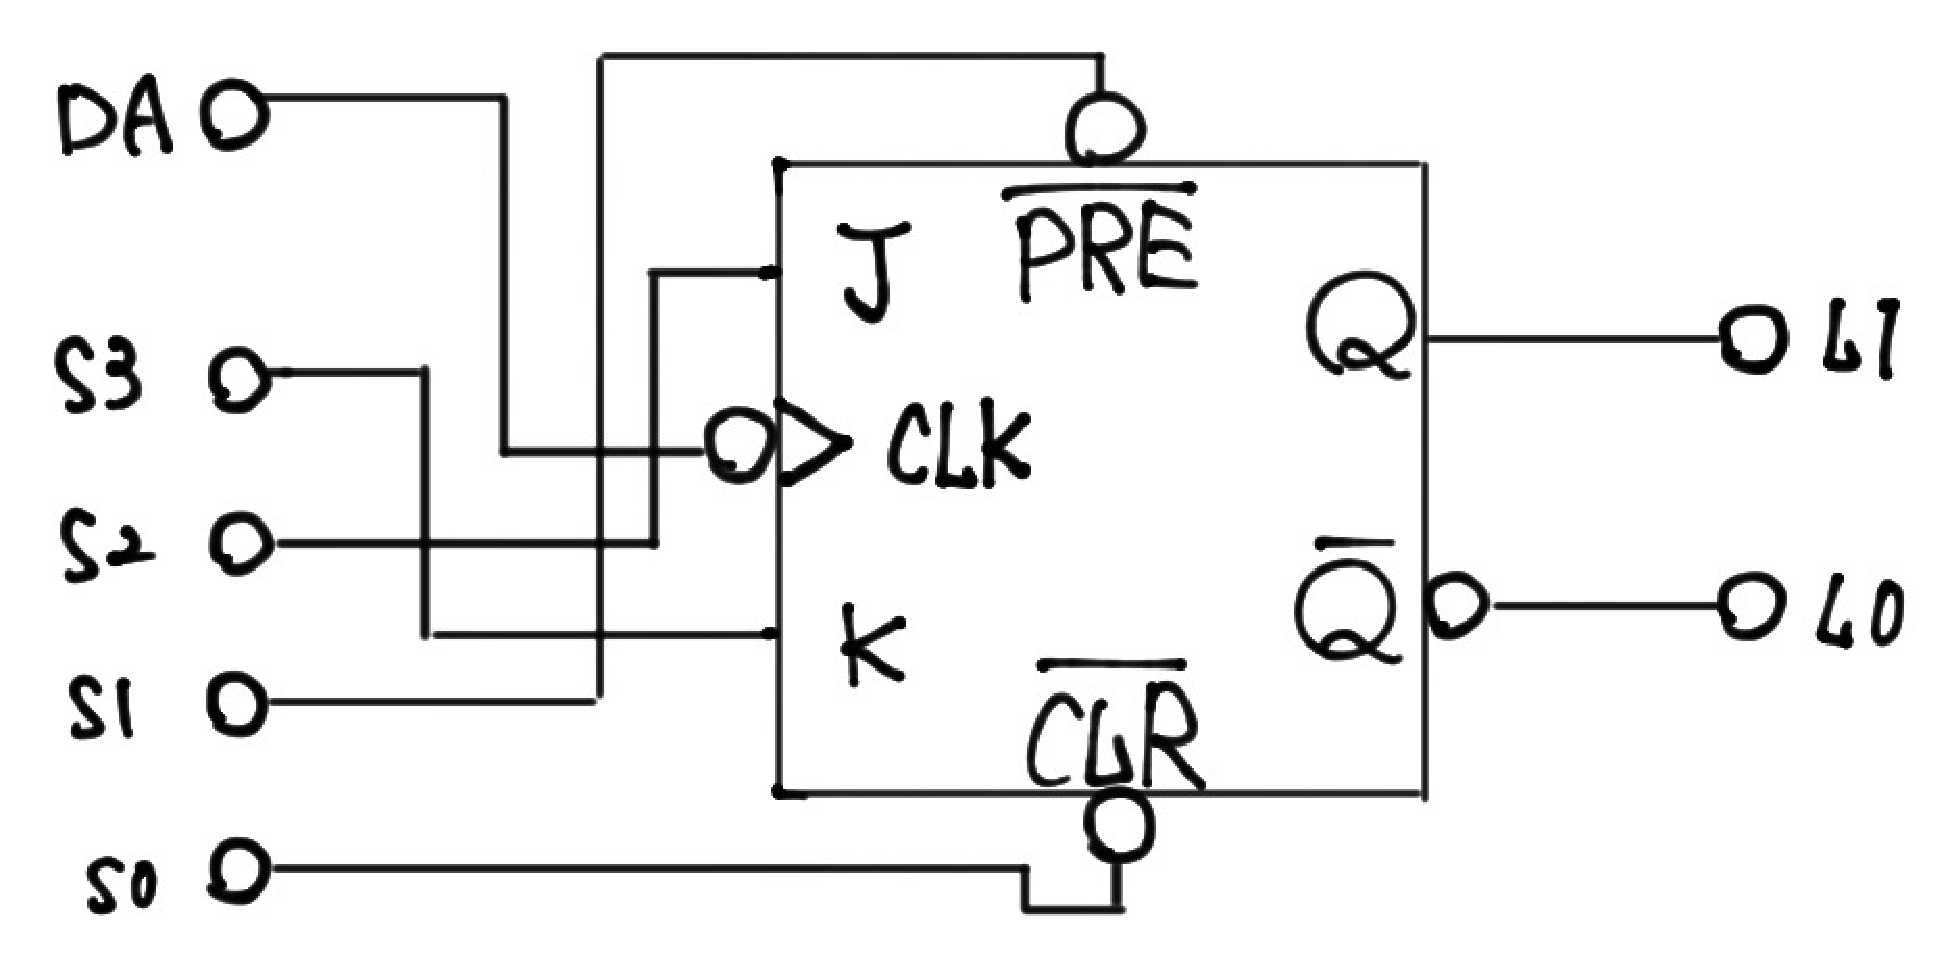
\includegraphics[width=8cm]{jkffcirc2} \\%%% ファイル名
				\end {center}
			\end{minipage}
		\end{tabular}
		\caption{J-Kフリップフロップ回路の回路図}%%% 表題
		\label{fig:JKFF}%%% ラベル
	\end{center}
\end{figure}
%
%
%
\begin{figure}[ht]
	\begin{center}
		\begin {tabular}{c}
			\begin{minipage}{8cm}
				\begin{center}
					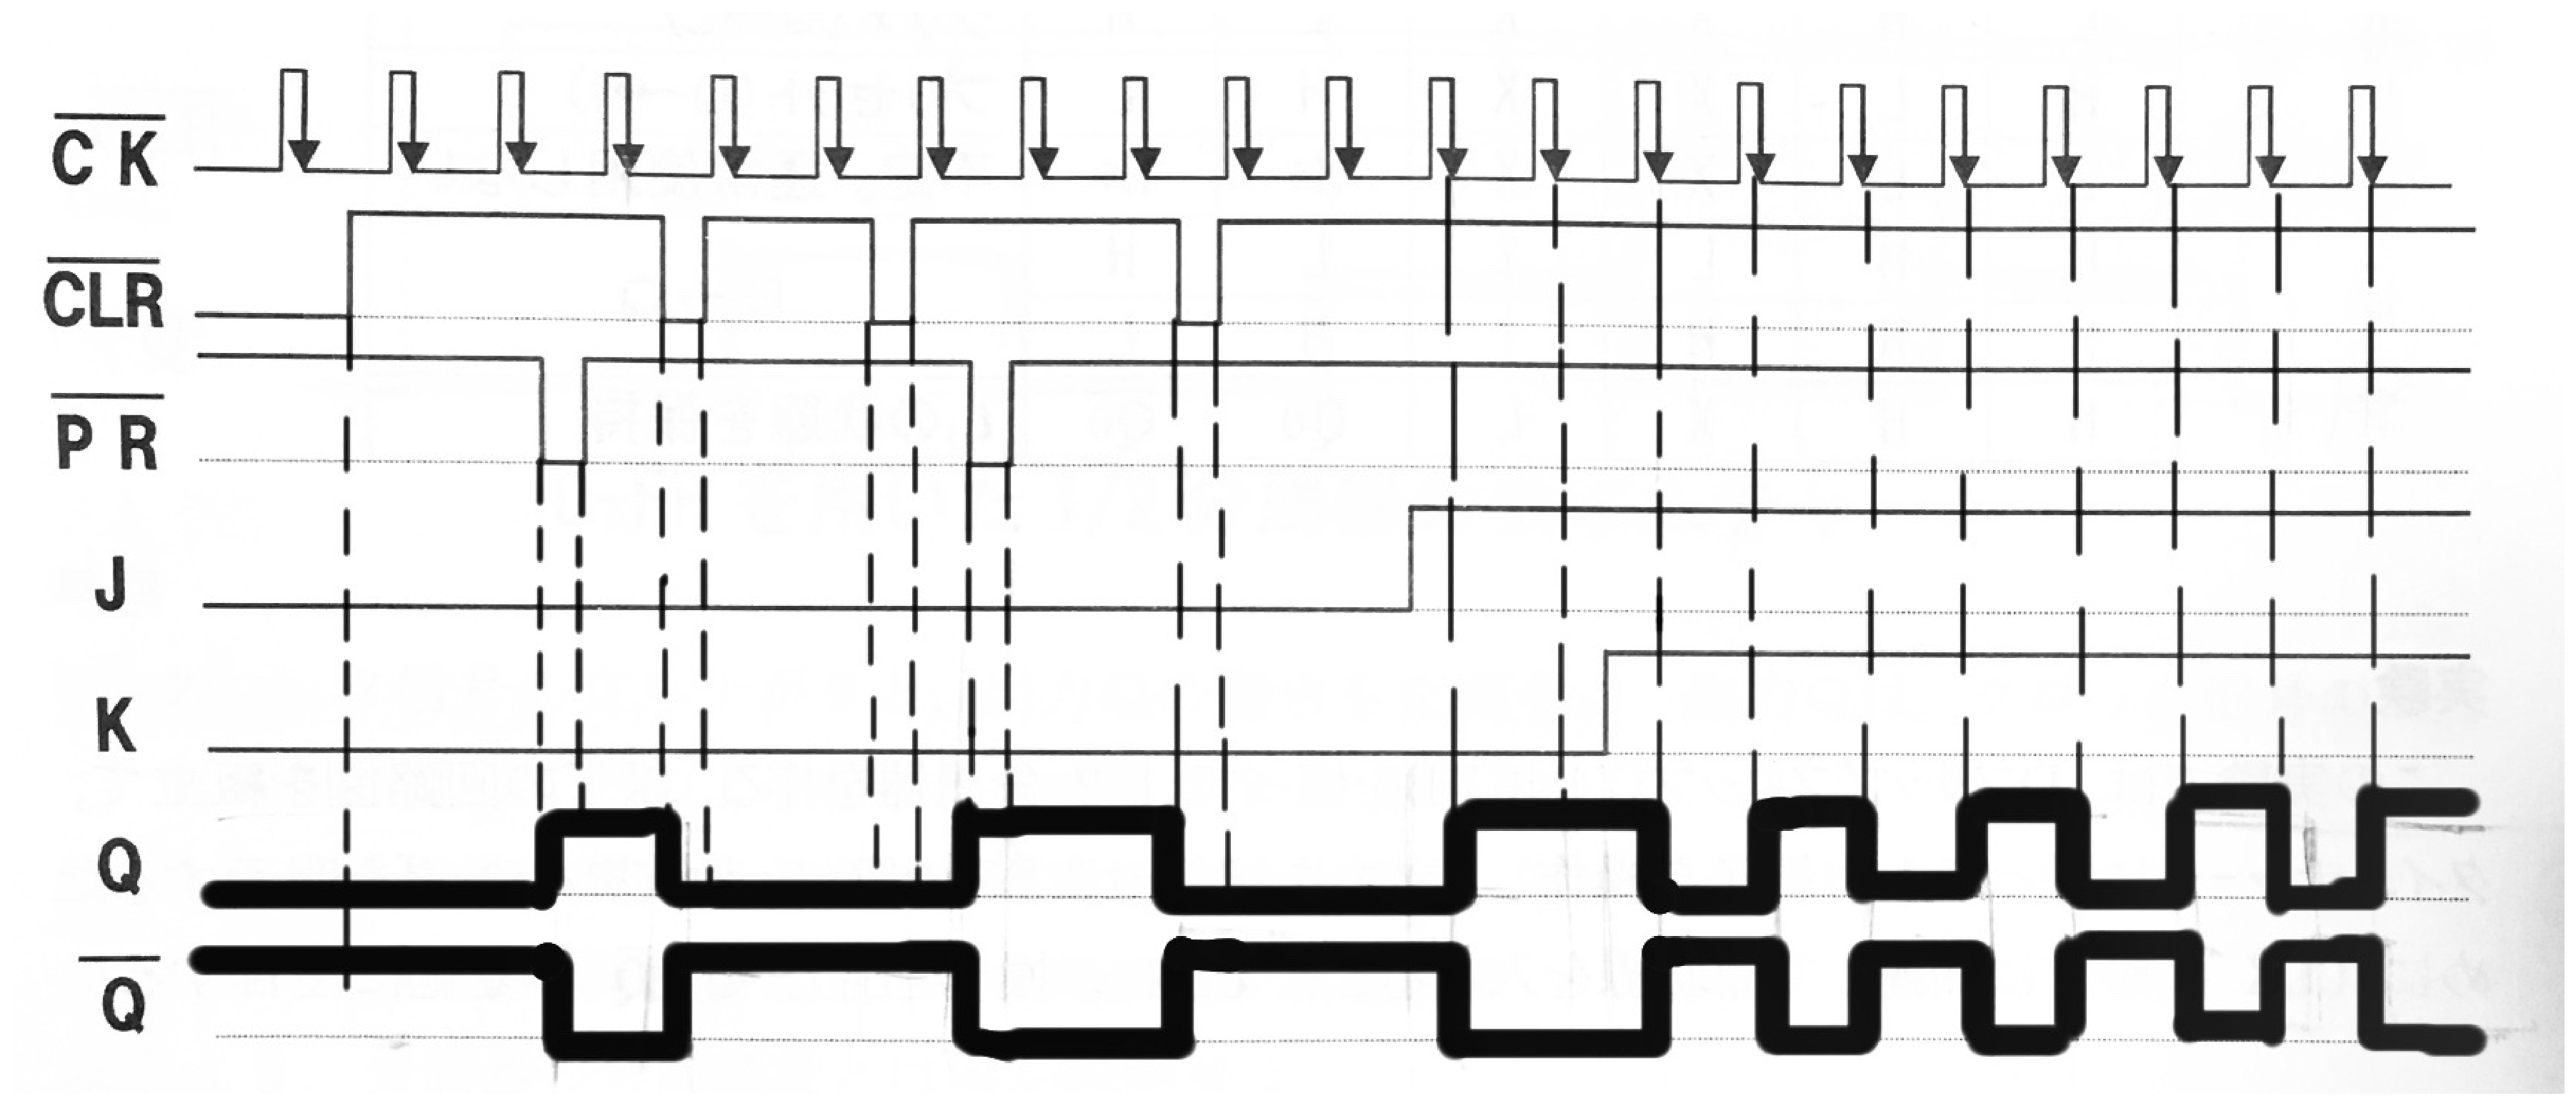
\includegraphics[width=8cm]{jkff2} \\%%% ファイル名
				\end {center}
			\end{minipage}
		\end{tabular}
		\caption{J-Kフリップフロップ回路のタイムチャート}%%% 表題
		\label{fig:JKFFTC}%%% ラベル
	\end{center}
\end{figure}
%
%
%
\begin{figure}[ht]
	\begin{center}
		\begin {tabular}{c}
			\begin{minipage}{8cm}
				\begin{center}
					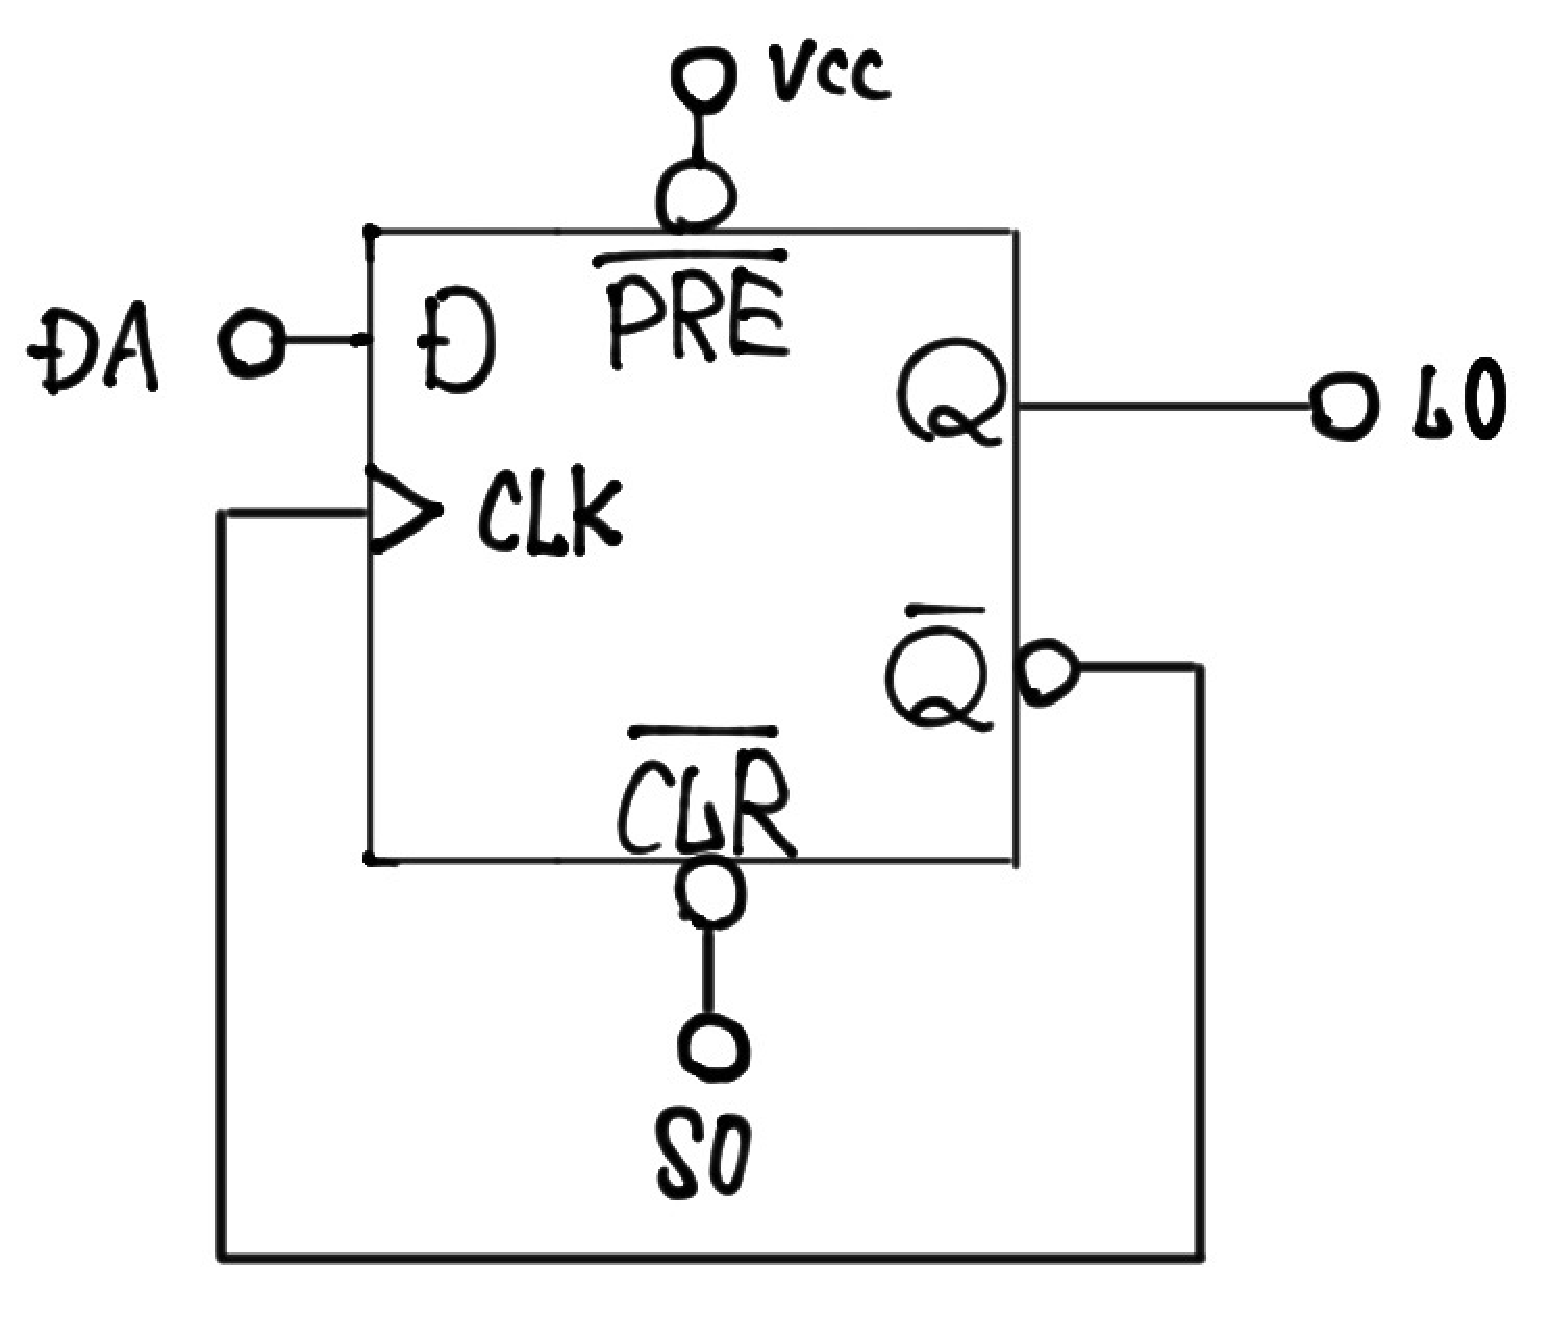
\includegraphics[width=8cm]{dffcirc2} \\%%% ファイル名
				\end {center}
			\end{minipage}
		\end{tabular}
		\caption{Dフリップフロップ回路の回路図}%%% 表題
		\label{fig:DFF}%%% ラベル
	\end{center}
\end{figure}
%
%
%
\begin{figure}[ht]
	\begin{center}
		\begin {tabular}{c}
			\begin{minipage}{8cm}
				\begin{center}
					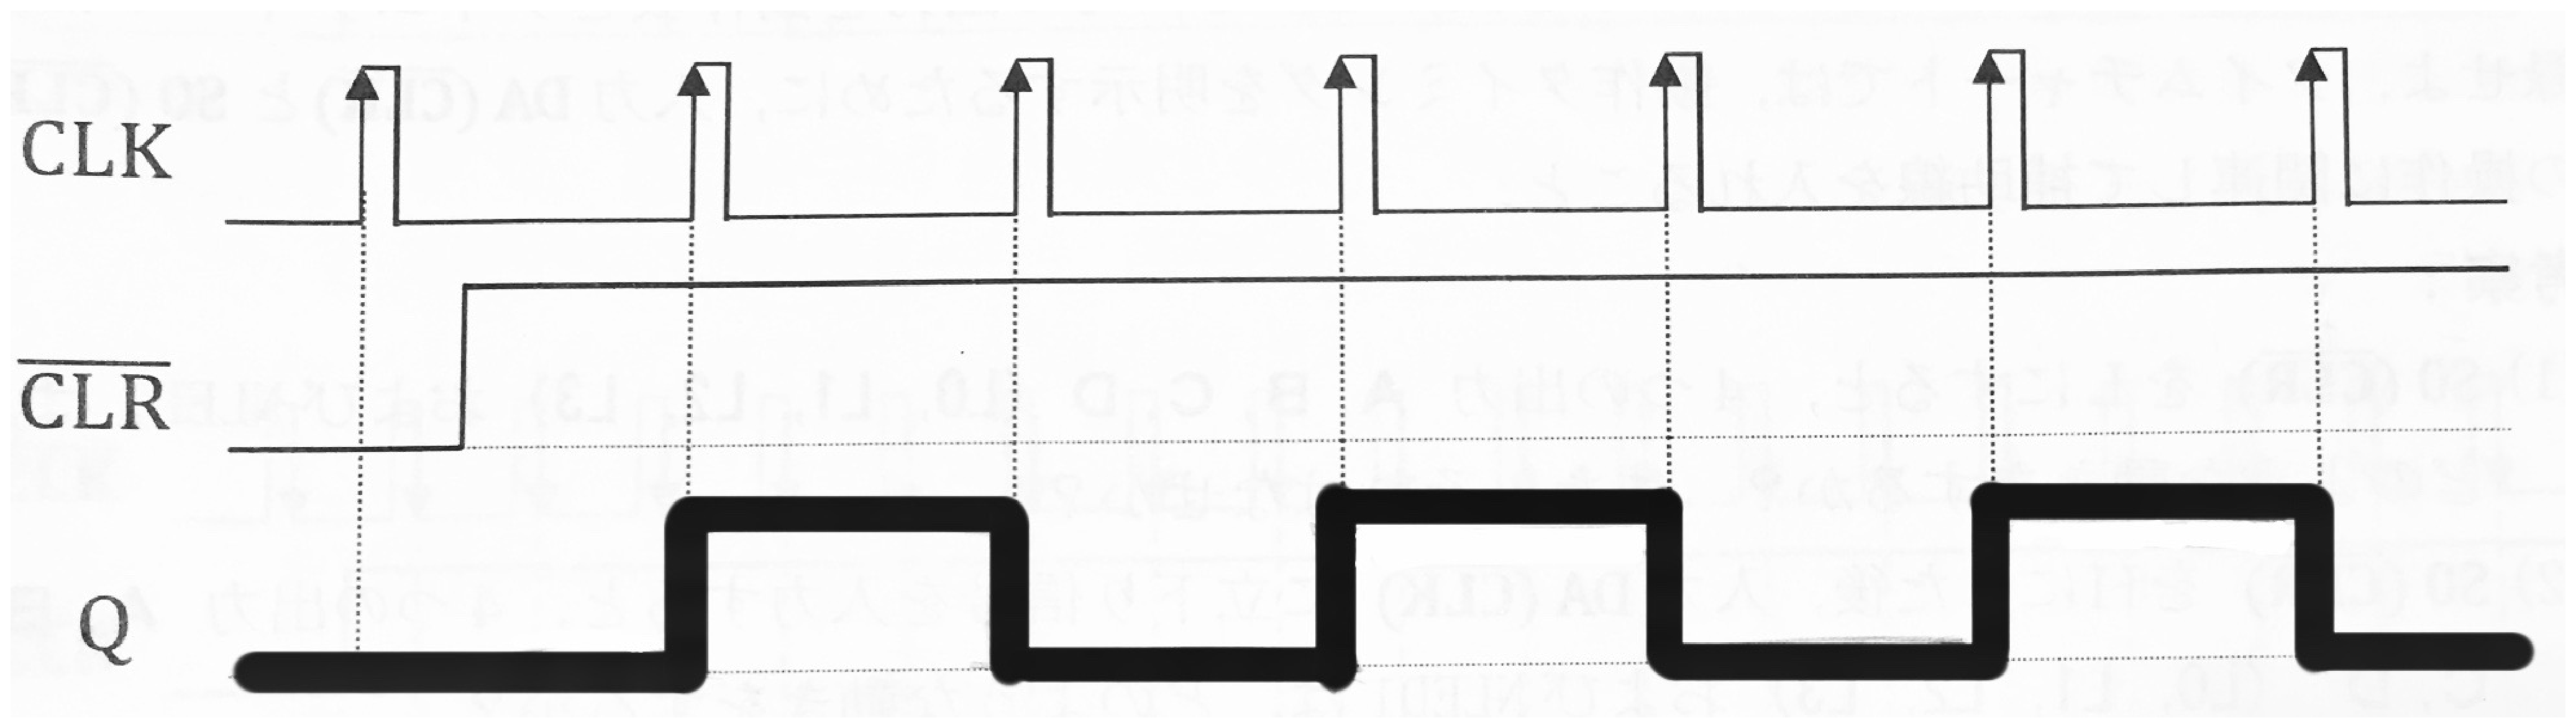
\includegraphics[width=8cm]{DFFTC} \\%%% ファイル名
				\end {center}
			\end{minipage}
		\end{tabular}
		\caption{Dフリップフロップ回路のタイムチャート}%%% 表題
		\label{fig:DFFTC}%%% ラベル
	\end{center}
\end{figure}
%
%
%
\begin{figure}[ht]
	\begin{center}
		\begin {tabular}{c}
			\begin{minipage}{12cm}
				\begin{center}
					\includegraphics[width=12cm]{16ctcir} \\%%% ファイル名
				\end {center}
			\end{minipage}
		\end{tabular}
		\caption{$16$進カウンタ回路の回路図}%%% 表題
		\label{fig:16Counter}%%% ラベル
	\end{center}
\end{figure}
%
%
%
\begin{figure}[ht]
	\begin{center}
		\begin {tabular}{c}
			\begin{minipage}{8cm}
				\begin{center}
					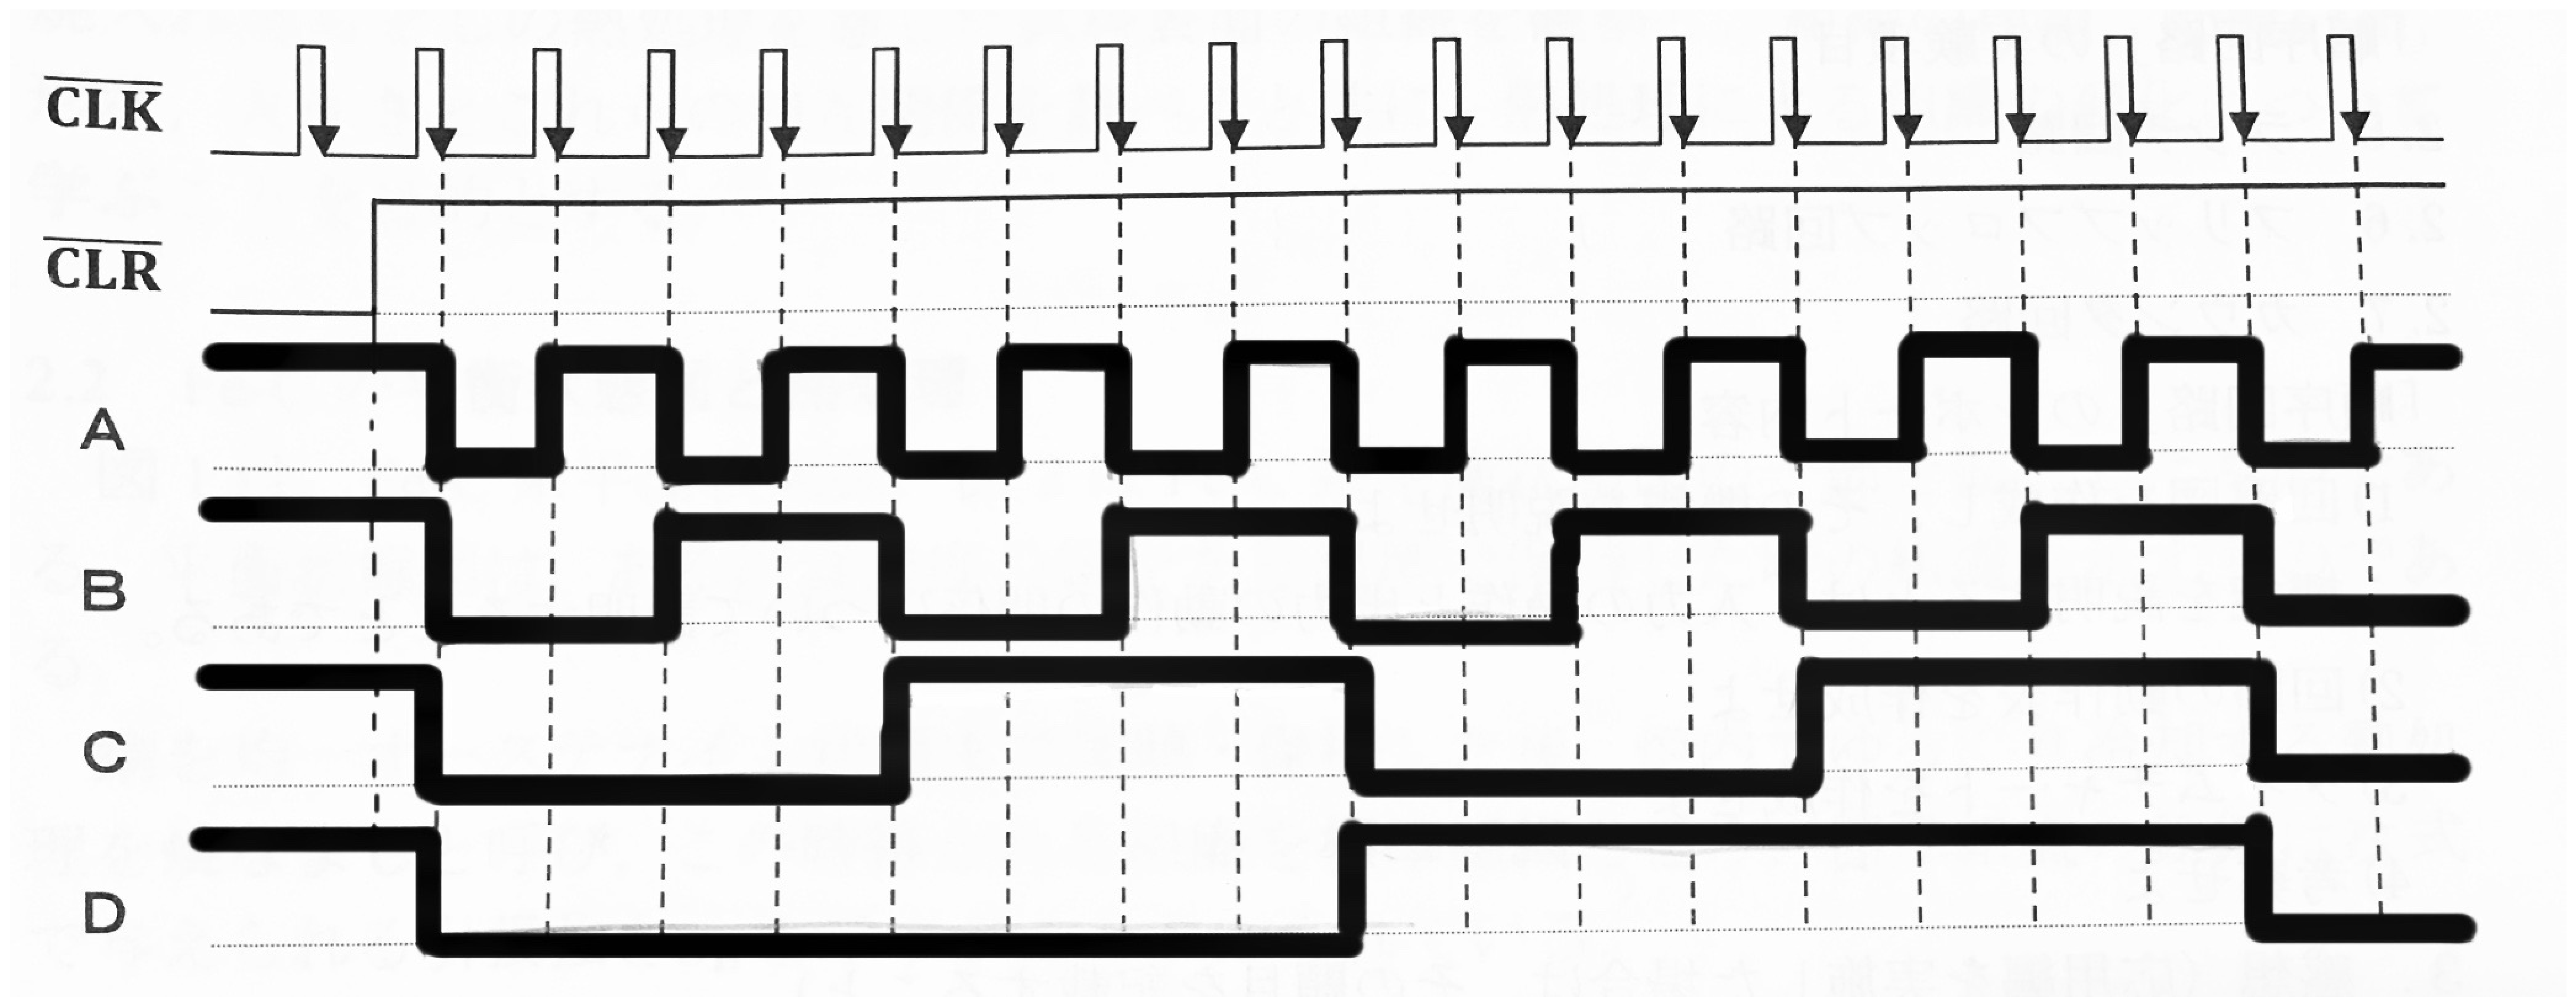
\includegraphics[width=8cm]{1111} \\%%% ファイル名
				\end {center}
			\end{minipage}
		\end{tabular}
		\caption{$16$進カウンタ回路のタイムチャート}%%% 表題
		\label{fig:16CounterTC}%%% ラベル
	\end{center}
\end{figure}
